\def\thedraft{2.1}

\author{Z. Akbar \and R.A. Badui \and J. Bono \and C. Bookwalter \and S. Chandavar \and V. Crede \and P. Eugenio \and J.T. Goetz \and L. Guo \and K. Hicks \and V. Kubarovsky \and M.C. Kunkel \and M. Paolone \and W. Phelps \and J.W. Price \and M. Saini \and C. Salgado \and D. Schott \and D.P. Weygand \and C. Zeoli}

\title{\desg{g12} Analysis Procedures, Statistics and Systematics}
\def\brieftitle{\desg{g12} Analysis Procedures}
\date{\today}

\documentclass[12pt,onecolumn,oneside,letterpaper]{article}
\usepackage{amsmath}
\usepackage{unicode-math}
\usepackage{fontspec}
\usepackage{xunicode}
\usepackage{xltxtra}
\usepackage{calc,bm,textcomp,latexsym,footmisc}
\usepackage{framed,url,verbatim}
\usepackage{longtable,multirow}
\usepackage[hang,small,bf]{caption}
\usepackage{subcaption}
\usepackage{graphicx}
\usepackage[usenames,dvipsnames]{xcolor}
\usepackage[margin=0.7in,top=1in,bottom=1in]{geometry}
\usepackage[export]{adjustbox}
\usepackage{fancyvrb}
% placeins package adds \FloatBarrier command to flush figures
% section option puts \FloatBarrier before every section
\usepackage[section]{placeins}
\usepackage[colorlinks]{hyperref}
\usepackage{sectsty}
	\chapterfont{\raggedright}
	\sectionfont{\raggedright}
	\subsectionfont{\raggedright}
	\subsubsectionfont{\raggedright}
\usepackage{setspace} % allows \<double,onehalf,single>spacing
	\singlespacing
	

\usepackage[backend=biber,texencoding=utf8,bibencoding=utf8,style=numeric-comp,sorting=none]{biblatex}
\addbibresource[datatype=bibtex]{bibliography/clas_general.bib}
\addbibresource[datatype=bibtex]{bibliography/clas_proposals.bib}
\addbibresource[datatype=bibtex]{bibliography/clas_theses.bib}
\addbibresource[datatype=bibtex]{bibliography/pdg.bib}
\addbibresource[datatype=bibtex]{bibliography/pol.bib}
\addbibresource[datatype=bibtex]{bibliography/pwa.bib}

\usepackage{fancyhdr}
\fancypagestyle{firststyle}
{
	\fancyhf{}
	\renewcommand{\headheight}{30pt}
	\renewcommand{\headrulewidth}{0pt}
	\fancyhead[R]{\large CLAS ANALYSIS 2017-101}
}
	
\setlength{\footskip}{0.3in}
\setmainfont[Ligatures=TeX]{Times New Roman}
%%% XITS Math Font
\setmathfont
[    Extension = .otf,
BoldFont = *bold,
]{xits-math}

\definecolor{DarkBlue}{rgb}{0,0.1,0.4}
\hypersetup{
	bookmarksnumbered,
	bookmarksopen=false,
	bookmarksopenlevel=\maxdepth,
	linkcolor=blue,
	urlcolor=DarkBlue,
	citecolor=green
}

\author{Z. Akbar \and R.A. Badui \and J. Bono \and C. Bookwalter \and S. Chandavar \and V. Crede \and P. Eugenio \and J.T. Goetz \and L. Guo \and K. Hicks \and V. Kubarovsky \and M.C. Kunkel \and M. Paolone \and W. Phelps \and J.W. Price \and M. Saini \and C. Salgado \and D. Schott \and D.P. Weygand \and C. Zeoli}

\title{\desg{g12} Analysis Procedures, Statistics and Systematics}
\def\brieftitle{\desg{g12} Analysis Procedures}
\newlength{\figwidth}
\setlength{\figwidth}{0.9\columnwidth}

\newlength{\qfigheight}
\setlength{\qfigheight}{0.25\textheight}

\newlength{\hfigheight}
\setlength{\hfigheight}{0.5\textheight}

\newcommand{\abbr}[1]{\textsc{\texttt{#1}}}
\newcommand{\desg}[1]{\texttt{#1}}
\newcommand{\prog}[1]{\texttt{#1}}

\newcommand{\todo}[1]{\textbf{\textcolor{Orange}{#1}}}

\def\Lqcd{\mathcal{L}_{\mathtt{QCD}}}
\def\qfield{\psi}
\def\qbarfield{\overline{\psi}}

\newcommand{\bank}[4]{$\mathtt{#1}^{#2}_{#3}\lbrack\mathtt{#4}\rbrack$}

\def\th{\textsuperscript{th}}
\def\ith{i\th}

\def\um{{\textmu}m}
\def\d{\mathrm{d}}

%\def\coloronline{(Color online.)\ }
\def\coloronline{}

%%% quarks
\def\uquark{\mathbf{u}}
\def\dquark{\mathbf{d}}
\def\squark{\mathbf{s}}

%%% particles
\def\photon{\gammaup}
\def\electron{\mathrm{e}^-}
\def\positron{\mathrm{e}^+}
\def\nucleon{\mathrm{N}}
\def\proton{\mathrm{p}}
\def\neutron{\mathrm{n}}
\def\pion{\piup}
\def\kaon{\mathrm{K}}
\def\hyperon{\mathrm{Y}}
\def\etameson{\etaup}
\def\omegameson{\omegaup}
\def\phimeson{\varphiup}
\def\rhomeson{\rhoup}

%%% TAGGER and RF related times
\def\trf{t_{\mathtt{RF}}}
\def\ttag{t_{\mathtt{TAG}}}
\def\ttagrf{t_{\mathtt{TAG,RF}}}
\def\tpho{t_\mathrm{photon}}
\def\tprop{t_\mathrm{prop}}
\def\ttrigoffset{t_{\mathrm{trigger-offset}}}

\def\dtpho{\Delta\tpho}

%%% BEAM energy
\def\ebeam{E_{\mathrm{beam}}}

%%% TOF Energy deposit
\def\etof{\frac{\mathrm{d}E}{\mathrm{d}x}(\mathtt{TOF})}
\def\varetof{\mathrm{d}E/\mathrm{d}x(\mathtt{TOF})}

%%% Beta
\def\betasttof{\beta_\mathtt{ST-TOF}}
\def\betatof{\beta_\mathtt{TOF}}
\def\betapid{\beta_\mathtt{PID}}

%%% path lengths
\def\lst{\ell_{\mathtt{ST}}}
\def\ltof{\ell_{\mathtt{TOF}}}
\def\lsttof{\ell_{\mathtt{ST-TOF}}}

%%% raw subsystem times
\def\tst{t_{\mathtt{ST}}}
\def\ttof{t_{\mathtt{TOF}}}
\def\dtsttof{\Delta t_{\mathrm{ST-TOF}}}

%%% vertex times
\def\tv{t_{\mathrm{vtx}}}
\def\tvtagrf{t_{\mathrm{vtx}}(\mathtt{TAG_{RF}})}
\def\tvtof{t_{\mathrm{vtx}}(\mathtt{TOF})}
\def\tvst{t_{\mathrm{vtx}}(\mathtt{ST})}
\def\tvpid{t_{\mathrm{vtx}}(\mathtt{PID})}

%%% delta vertex times
\def\dtvst{\Delta t_\mathrm{vtx}(\mathtt{TOF-ST})}
\def\dtvpid{\Delta t_\mathrm{vtx}(\mathtt{TOF-PID})}

\def\adcst{\mathtt{ADC}_{\mathtt{ST}}}

\def\M{\mathrm{M}}
\def\MM{\mathrm{MM}}

%%% units
\def\GeV{\mathrm{GeV}}
\def\ns{\mathrm{ns}}

\newcommand{\bra}[1]{\left<#1\right|}
\newcommand{\ket}[1]{\left|#1\right>}
\newcommand{\braket}[2]{\left<#1\middle|#2\right>}

\newcommand*\midhrulefill{%
    \leavevmode\leaders\hrule depth-2pt height 2.4pt\hfill\kern0pt
}


%%%%%%%%%%%%%%%%%%%%%%%%%%%%%%%%%%%%%%%%%%%%%%%%%%%%%%%%%%%%%%%%%%%%%%%

\begin{document}

%%% define the footnote symbol. Can be one of these:
    %\fnsymbol   *, + ...
    %\arabic     1, 2 ...
    %\roman      i, ii ...
    %\Roman      I, II ...
    %\alph       a, b ...
    %\Alph       A, B ...
\renewcommand{\thefootnote}{\fnsymbol{footnote}}

\pagestyle{headings}
%\renewcommand{\sectionmark}[1]{\markboth{#1}{}}

\pdfbookmark[1]{Title}{title}
\maketitle

\pdfbookmark[1]{Table of Contents}{toc}
    \tableofcontents \clearpage
%\phantomsection \addcontentsline{toc}{section}{List of Figures}
    %\listoffigures \clearpage
%\phantomsection \addcontentsline{toc}{section}{List of Tables}
    %\listoftables \clearpage

\begin{abstract}
This document serves to summarize all information needed to process and analyze data from the \abbr{CLAS} \desg{g12} experiment taken in the summer of 2008. This was a high-luminosity, high-energy real-photon run with a 65~nA circularly polarized beam, 40~cm unpolarized $\ell$H$_2$ target and an $\ebeam$ up to 5.7~GeV. The associated proposals, and therefore the trigger, focused on the high-energy part of the tagger, and though it was not part of the original proposals, the Cherenkov was active for most of the run.
\end{abstract}

\section{\label{sec:summary}Summary of Running Conditions}

This document is organized as follows. Section~\ref{sec:summary} has basic information about the \desg{g12} run, including the physics goals. Section~\ref{sec:calib} describes the calibrations; it is quite long and uses standard \abbr{CLAS} procedures. One item of note is that the beam current was high for \abbr{CLAS}, typically about 60 nA. Of course, the background rate goes quadratically with beam current, and so the \desg{g12} data have more background yet the calibration procedures still work. Section~\ref{sec:data} provides the cooking procedures, as well as the momentum and beam-energy corrections. Since \desg{g12} also had a lepton trigger, Section~\ref{sec:data.lepton} gives additional information relevant to the lepton detection using the CC and EC. Section~\ref{sec:flux} has a straight-forward description of the beam flux, using the \prog{gflux} method with the \verb+–c+ option (clock-based DAQ). Section~\ref{sec:sim} provides the procedures for simulations, including all command-line options (some a1c options are specific to BOS files made from simulations). This section also has specific information for \desg{g12}, such as the fiducial cuts and simulations of the \desg{g12} trigger. Finally, Sections~\ref{sec:resonances} and \ref{sec:xsec} together show that the world data on cross sections for at least two reactions (ω meson production and K$^+$ Λ production) agree well with previously reported world data. This gives us confidence that the calibrations, energy corrections, beam flux and simulations are being done correctly.

The goal of this document is to provide a basis for individual analyses of \desg{g12} data to undergo a shortened analysis review. In other words, if the procedures here are followed also in individual analyses, then the review committees can focus on the cuts and systematics specific to the final state of an individual analysis, with confidence that the calibrations, corrections, etc., have already been reviewed.

The \desg{g12} experiment contained several analyses where the main goal was to search for resonances in the multi-particle final state by performing partial wave analysis. These analyses\cite{clas.thesis.bookwalter, clas.thesis.schott} do not require absolute normalization and therefore several steps discussed below were skipped. For a general discussion of the PWA procedure by \desg{g12} Ref.~\cite{pwa.salgado2014}. We do however provide details for analyses that do want this normalization for cross sections and upper limits later in this document.

The \desg{g12} experiment was a high-luminosity, high-energy real-photon run for \abbr{CLAS}. The electron beam current was 60--65~nA on the 40~cm $\ell$H$_2$ target. A total of $26\times 10^8$ triggers were recorded using several of the 12 available trigger bits. The ``production trigger'' required two prongs (start-counter and time-of-flight coincidence) in two different sectors and in coincidence with a tagger hit at or above 3.6~GeV. There was secondary trigger which required three prongs, again in different sectors, regardless of tagger hits. The running conditions are summarized in Table~\ref{tab:runconditions}. There were three proposals associated with this experiment which are listed here:
\begin{itemize}
    \item \href{https://misportal.jlab.org/ul/ul_office/experimentdb/view_experiment_detail.cfm?paperid=PR-04-005}{\fullcite{clas.proposal.hyclas}}
    \item \href{https://misportal.jlab.org/ul/ul_office/experimentdb/view_experiment_detail.cfm?paperid=PR-04-017}{\fullcite{clas.proposal.superg}}
    \item \href{https://misportal.jlab.org/ul/ul_office/experimentdb/view_experiment_detail.cfm?paperid=PR-08-003}{\fullcite{clas.proposal.pion}}
\end{itemize}

In addition to this document, there is a wealth of information to be found in the wiki pages at
\begin{center}
    \url{http://clasweb.jlab.org/rungroups/g12/wiki}
\end{center}
which has served as a repository for all things related to the \desg{g12} experiment. The dissertations associated with this experiment contain a lot of information as well:

\begin{itemize}
    \item \href{http://www.jlab.org/Hall-B/general/thesis/Goetz_thesis.pdf}{\fullcite{clas.thesis.goetz}}
    \item \href{http://www.jlab.org/Hall-B/general/thesis/Bookwalter_thesis.pdf}{\fullcite{clas.thesis.bookwalter}}
    \item \href{http://www.jlab.org/Hall-B/general/thesis/Schott_thesis.pdf}{\fullcite{clas.thesis.schott}}
    \item \href{http://www.jlab.org/Hall-B/general/thesis/MSaini_thesis.pdf}{\fullcite{clas.thesis.saini}}
    \item \href{http://www.jlab.org/Hall-B/general/thesis/Bono_thesis.pdf}{\fullcite{clas.thesis.bono}}
    \item \href{http://www.jlab.org/Hall-B/general/thesis/Kunkel_thesis.pdf}{\fullcite{clas.thesis.kunkel}}
    \item \href{http://www.jlab.org/Hall-B/general/thesis/Chandavar_thesis.pdf}{\fullcite{clas.thesis.chandavar}}
\end{itemize}


\begin{table}[htpb]
\begin{center}

\begin{minipage}{0.8\textwidth}

\caption{\label{tab:runconditions}The running conditions of the \desg{g12} experiment.}
\begin{center}
\begin{tabular}{lc}

\hline \hline

$\ebeam$ of photon & 5.715~GeV \\
Beam Polarization & Circular \\
e$^-$ Current & 60--65~nA \\
Tagger Range & 5\% - 95\% of e$^-$ energy \\
Tagger Trigger Range & 3.6--5.441~GeV \\
Torus Magnet & $\frac{1}{2} B_\mathrm{max}$ (1930~A) \\
Target Length & 40~cm \\
Target Center ($z$ location) & $-90$~cm \\
Target Material & $\ell$H$_2$ \\
Target Polarization & None \\
Start Counter Offset & 0~cm \\
Radiator Thickness & $10^{-4}$~radiation~lengths \\
Collimator Radius & 6.4~mm \\

\hline \hline

\end{tabular}
\end{center}

\end{minipage}

\end{center}
\end{table}


\subsection{\label{sec:summary.trigger}Trigger Configurations}

The \desg{g12} experiment was the first Hall \desg{B} run-period to implement field programmable gate array (\abbr{FPGA}) processors to handle the trigger logic of the \abbr{abbr{CLAS}} detector (see Sec.~\ref{sec:clas.daq}). With this new \abbr{FPGA}-powered triggering system, came the ability to modify the trigger quickly during the experiment. While potentially dangerous --- these changes must be accounted for in total-cross-sectional analyses for example --- this allowed the group to tune the trigger to get the highest possible rate of physical events.

The trigger bits used during the \desg{g12} running period are defined in Tables~\ref{tab:data.trig.conf.1}, \ref{tab:data.trig.conf.2} and \ref{tab:data.trig.conf.3}. They generally consisted of a number of tracks which were the coincidence of any one of the four start counter paddles and any of the 57 time-of-flight paddles in a given sector as discussed in Sec.~\ref{sec:clas.daq}. The hardware and configuration did not allow triggering on two tracks in the same sector because there were only six signals coming from the \abbr{TOF} --- one for each sector. The coincidence of these tracks with the photon tagger, called the ``Master-\abbr{OR},'' is defined in Table~\ref{tab:data.trig.mor}.

\begin{table}
\begin{minipage}{\textwidth}
\begin{center}
\begin{singlespacing}

\caption[Trigger Configuration 1]{\label{tab:data.trig.conf.1}Trigger configuration for \desg{g12} runs from 56363 to 56594 and 56608 to 56647. (\abbr{ST}$\times$\abbr{TOF})$_{i}$ indicates a single \emph{prong} which is a trigger-level track defined as a coincidence between a start counter and time-of-flight hit in the \ith\ sector or any sector if the subscript index, $i$, is not specified. An added $\times$2 or $\times$3 indicates the coincidence of multiple \emph{prongs} which are not in the same sector. \abbr{MORA} and \abbr{MORB} represent coincidences with tagger hits within a certain energy range as specified in Table~\ref{tab:data.trig.mor}.}

\begin{tabular}{cccc}

\hline \hline

\multicolumn{4}{c}{\desg{g12} runs 56363--56594, 56608--56647} \\

\hline

bit & definition & L2 multiplicity & prescale \\

\hline

1 & \abbr{MORA}$\cdot$(\abbr{ST}$\times$\abbr{TOF})$_{1}\cdot$(\abbr{ST}$\times$\abbr{TOF}) & -- & 1 \\
2 & \abbr{MORA}$\cdot$(\abbr{ST}$\times$\abbr{TOF})$_{2}\cdot$(\abbr{ST}$\times$\abbr{TOF}) & -- & 1 \\
3 & \abbr{MORA}$\cdot$(\abbr{ST}$\times$\abbr{TOF})$_{3}\cdot$(\abbr{ST}$\times$\abbr{TOF}) & -- & 1 \\
4 & \abbr{MORA}$\cdot$(\abbr{ST}$\times$\abbr{TOF})$_{4}\cdot$(\abbr{ST}$\times$\abbr{TOF}) & -- & 1 \\
5 & \abbr{MORA}$\cdot$(\abbr{ST}$\times$\abbr{TOF})$_{5}\cdot$(\abbr{ST}$\times$\abbr{TOF}) & -- & 1 \\
6 & \abbr{MORA}$\cdot$(\abbr{ST}$\times$\abbr{TOF})$_{6}\cdot$(\abbr{ST}$\times$\abbr{TOF}) & -- & 1 \\
7 & \abbr{ST}$\times$\abbr{TOF} & -- & 1 \\
8 & \abbr{MORA}$\cdot$(\abbr{ST}$\times$\abbr{TOF})$\times$2 & -- & 1 \\
11\footnote{bit 11 and \abbr{MORB} were included in the trigger starting with run 56519.} & \abbr{MORB}$\cdot$(\abbr{ST}$\times$\abbr{TOF})$\times$2 & -- & 1 \\
12 & (\abbr{ST}$\times$\abbr{TOF})$\times$3 & -- & 1 \\

\hline \hline

\end{tabular}

\end{singlespacing}
\end{center}
\end{minipage}
\end{table}
 % label: tab:data.trig.conf.1

\begin{table}
\begin{minipage}{\textwidth}
\begin{center}
\begin{singlespacing}

\caption[Trigger Configuration 2]{\label{tab:data.trig.conf.2}Trigger configuration for \desg{g12} runs from 56595 to 56607 and 56648 to 57323. (\abbr{EC}$\times$\abbr{CC}) represents a coincidence between the electromagnetic calorimeter and the \v{C}erenkov subsystems within a single sector using the thresholds as described in Table~\ref{tab:data.ecccthresh}. \abbr{ECP} represents the \emph{photon} threshold trigger from the \abbr{EC}. See Table~\ref{tab:data.trig.conf.1} for other explanatory details.}

\begin{tabular}{cccc}

\hline \hline

\multicolumn{4}{c}{\desg{g12} runs 56595--56607, 56648--57323 } \\

\hline

bit & definition & L2 multiplicity\footnote{Level 2 triggering was turned off on all bits for runs 56605, 56607 and 56647.} & prescale \\

\hline

1 & \abbr{MORA}$\cdot$(\abbr{ST}$\times$\abbr{TOF}) & 1 & 1000/300\footnote{Prescaling for bits 1 and 4 were 1000 for runs prior to 56668 at which point they both were changed to 300.} \\
2 & \abbr{MORA}$\cdot$(\abbr{ST}$\times$\abbr{TOF})$\times$2 & 2/--\footnote{Level 2 triggering of bit 2 was set to 2 for runs prior to 56665 at which point it was turned off.} & 1 \\
3 & \abbr{MORB}$\cdot$(\abbr{ST}$\times$\abbr{TOF})$\times$2 & 2 & 1 \\
4 & \abbr{ST}$\times$\abbr{TOF} & 1 & 1000/300 \\
5 & (\abbr{ST}$\times$\abbr{TOF})$\cdot$\abbr{ECP}$\times$2 & 1 & 1 \\
6 & (\abbr{ST}$\times$\abbr{TOF})$\cdot$(\abbr{EC}$\times$\abbr{CC}) & 2 & 1 \\
7 & \abbr{MORA}$\cdot$(\abbr{ST}$\times$\abbr{TOF})$\cdot$(\abbr{EC}$\times$\abbr{CC}) & -- & 1 \\
8 & \abbr{MORA}$\cdot$(\abbr{ST}$\times$\abbr{TOF})$\times$2 & -- & 1 \\
11 & (\abbr{EC}$\times$\abbr{CC})$\times$2 & -- & 1 \\
12 & (\abbr{ST}$\times$\abbr{TOF})$\times$3 & -- & 1 \\

\hline \hline

\end{tabular}

\end{singlespacing}
\end{center}
\end{minipage}
\end{table}

 % label: tab:data.trig.conf.2

\begin{table}
\begin{minipage}{\textwidth}
\begin{center}
\begin{singlespacing}

\caption[Trigger Configuration for Single-sector Runs]{\label{tab:data.trig.conf.3}Trigger configuration for the single-sector runs of \desg{g12}. Trigger bits 7--12 were not used for these runs. See Table~\ref{tab:data.trig.conf.1} for explanatory details.}

\begin{tabular}{cccc}

\hline \hline

bit & definition & L2 multiplicity & prescale \\

\hline

1 & \abbr{MORA}$\cdot$(\abbr{ST}$\times$\abbr{TOF})$_{1}$ & sector 1 & 1 \\
2 & \abbr{MORA}$\cdot$(\abbr{ST}$\times$\abbr{TOF})$_{2}$ & sector 2 & 1 \\
3 & \abbr{MORA}$\cdot$(\abbr{ST}$\times$\abbr{TOF})$_{3}$ & sector 3 & 1 \\
4 & \abbr{MORA}$\cdot$(\abbr{ST}$\times$\abbr{TOF})$_{4}$ & sector 4 & 1 \\
5 & \abbr{MORA}$\cdot$(\abbr{ST}$\times$\abbr{TOF})$_{5}$ & sector 5 & 1 \\
6 & \abbr{MORA}$\cdot$(\abbr{ST}$\times$\abbr{TOF})$_{6}$ & sector 6 & 1 \\

\hline \hline

\end{tabular}

\end{singlespacing}
\end{center}
\end{minipage}
\end{table}

 % label: tab:data.trig.conf.3

\begin{table}
\begin{center}
\begin{singlespacing}

\caption[Trigger Configuration (Tagger)]{\label{tab:data.trig.mor}Master-\abbr{OR} definitions for \desg{g12}. The \abbr{TDC} counters were used in the trigger and since each of these corresponds to several energy paddles, the energies given here are approximate. $T$-counter number 1 corresponds to the highest energy photon of approximately 5.4~GeV. Both \abbr{MORA} and \abbr{MORB} are referenced in terms of the trigger logic in Tables~\ref{tab:data.trig.conf.1}, \ref{tab:data.trig.conf.2} and \ref{tab:data.trig.conf.3}. The \emph{single-sector} runs are listed in Table~\ref{tab:data.cook.singlesecruns}.}

\begin{tabular}{c|cc|cc}

\hline \hline

          & \multicolumn{2}{c|}{\abbr{MORA}} & \multicolumn{2}{c}{\abbr{MORB}} \\
run range & $T$-counters & energy (GeV)     & $T$-counters & energy (GeV) \\

\hline

56363--56400 & 1--47 & 1.7--5.4 & -- & -- \\
56401--56518 & 1--25 & 3.6--5.4 & -- & -- \\
56519--57323 & 1--19 & 4.4--5.4 & 20--25 & 3.6--4.4 \\

\hline

\emph{single-sector} & 1--31 & 3.0--5.4 & -- & -- \\

\hline \hline

\end{tabular}

\end{singlespacing}
\end{center}
\end{table}
 % label:  tab:data.trig.mor

There were two sets of thresholds for the \abbr{EC} labeled \emph{photon} and \emph{electron}. These labels did not mean photon or electron specifically, but were considered a first-order approximation. The actual particle identification was done much later in the analysis of the reconstructed data. The thresholds for the \abbr{CC} and \abbr{EC} during the \desg{g12} running period are shown in Table~\ref{tab:data.ecccthresh}.

\begin{table}
\begin{center}
\begin{singlespacing}

\caption[\abbr{EC} and \abbr{CC} Trigger Thresholds]{\label{tab:data.ecccthresh}Threshold values for the electromagnetic calorimeter (\abbr{EC}) and \v{C}erenkov counter (\abbr{CC}) during the \g12 running period. \abbr{EC} thresholds are shown as \emph{inner}/\emph{total}, and \abbr{CC} thresholds are shown as \emph{left}/\emph{right}.}

\begin{tabular}{cc|c}

\hline \hline

\multicolumn{2}{c|}{\abbr{EC}} & \multirow{2}{*}{\abbr{CC}} \\

\emph{photon} & \emph{electron} \\


\hline

50/100~mV & 60/80~mV & 20/20~mV \\
150/300~MeV & 180/240~MeV & $\sim$0.4~photo-electrons \\

\hline \hline

\end{tabular}

\end{singlespacing}
\end{center}
\end{table}
 % label: tab:data.ecccthresh

\FloatBarrier

\subsection{\label{sec:summary.runs}Lists of Runs}

The runs for this experiment range from 56855 to 57317 inclusive. The runs that made it into Tables.~\ref{tab:data.cook.prodruns} and \ref{tab:data.cook.singlesecruns} qualified upon success of reconstructing final-state hadrons using the cooking program's default particle identification in coordination with the hand-written notes by the shift takers. Other runs of note include those used specifically for calibration in Table~\ref{tab:data.cook.org.runs} and normalization, zero-field and empty-target runs in Table~\ref{tab:data.calibruns}.

\begin{center}
\begin{singlespacing}
\begin{longtable}{lr|lr|lr}
\caption[Production Run List]{\label{tab:data.cook.prodruns}List of successfully reconstructed production runs and their beam currents in nA.} \\

\hline \hline
\multicolumn{2}{l|}{runs} & \multicolumn{2}{l|}{runs} & \multicolumn{2}{l}{runs} \\
\multicolumn{2}{r|}{current (nA)} & \multicolumn{2}{r|}{current (nA)} & \multicolumn{2}{r}{current (nA)} \\
\hline
\endfirsthead

\multicolumn{6}{l}{\scriptsize continued from previous page.} \\
\hline
\multicolumn{2}{l|}{runs} & \multicolumn{2}{l|}{runs} & \multicolumn{2}{l}{runs} \\
\multicolumn{2}{r|}{current (nA)} & \multicolumn{2}{r|}{current (nA)} & \multicolumn{2}{r}{current (nA)} \\
\hline
\endhead

\hline
\multicolumn{6}{r}{\scriptsize continued on next page.} \\
\endfoot

\hline \hline
\endlastfoot

56363 & 20 & 56605 & 60 & 56900-56908 & 60 \\
56365 & 30 & 56608-56612 & 60 & 56914-56919 & 60 \\
56369 & 30 & 56614-56618 & 60 & 56921-56922 & 60 \\
56384 & 5 & 56620-56628 & 60 & 56923 & 65 \\
56386 & 20 & 56630-56636 & 60 & 56924 & 70 \\
56401 & 50 & 56638-56644 & 60 & 56925 & 80 \\
56403 & 70 & 56646 & 60 & 56926-56930 & 60 \\
56404 & 60 & 56653-56656 & 60 & 56932 & 60 \\
56405 & 50 & 56660-56661 & 60 & 56935-56940 & 60 \\
56406 & 40 & 56665-56670 & 60 & 56948-56956 & 60 \\
56408 & 80 & 56673-56675 & 60 & 56958 & 60 \\
56410 & 90 & 56679-56681 & 60 & 56960-56975 & 60 \\
56420-56422 & 5 & 56683 & 60 & 56977-56980 & 60 \\
56435 & 5 & 56685-56696 & 60 & 56992-56994 & 60 \\
56436 & 15 & 56700-56708 & 60 & 56996-57006 & 60 \\
56441 & 35 & 56710-56724 & 60 & 57008-57017 & 60 \\
56442 & 30 & 56726-56744 & 60 & 57021-57023 & 60 \\
56443 & 20 & 56748-56750 & 60 & 57025-57027 & 60 \\
56445-56450 & 60 & 56751-56768 & 65 & 57030-57032 & 60 \\
56453-56459 & 60 & 56770-56772 & 65 & 57036-57039 & 60 \\
56460-56462 & 70 & 56774-56778 & 65 & 57062-57069 & 60 \\
56465 & 70 & 56780-56784 & 65 & 57071-57073 & 60 \\
56467-56472 & 70 & 56787-56788 & 65 & 57075-57080 & 60 \\
56478-56483 & 70 & 56791-56794 & 65 & 57095-57097 & 60 \\
56485-56487 & 70 & 56798-56802 & 65 & 57100-57103 & 60 \\
56489-56490 & 70 & 56805-56815 & 65 & 57106-57108 & 60 \\
56499 & 70 & 56821-56827 & 65 & 57114-57128 & 60 \\
56501 & 60 & 56831-56834 & 65 & 57130-57152 & 60 \\
56503 & 57 & 56838-56839 & 65 & 57159-57168 & 60 \\
56504 & 56 & 56841-56845 & 65 & 57170-57185 & 60 \\
56505-56506 & 40 & 56849 & 65 & 57189-57229 & 60 \\
56508-56510 & 60 & 56853-56862 & 65 & 57233-57236 & 60 \\
56513-56517 & 60 & 56864 & 65 & 57249-57253 & 60 \\
56519 & 60 & 56865-56866 & 60 & 57255-57258 & 60 \\
56521-56542 & 60 & 56870 & 65 & 57260-57268 & 60 \\
56545-56550 & 60 & 56874-56875 & 60 & 57270-57288 & 60 \\
56555-56556 & 60 & 56877 & 60 & 57290-57291 & 60 \\
56561-56564 & 60 & 56879 & 60 & 57293-57312 & 60 \\
56573-56583 & 60 & 56897-56898 & 60 & 57317 & 60 \\
56586-56593 & 60 & 56899 & 65 & & \\

\end{longtable}
\end{singlespacing}
\end{center}
 % label:  tab:data.cook.prodruns

\begin{table}
\begin{minipage}{\textwidth}
\begin{center}
\begin{singlespacing}

\caption[Single-sector Run List]{\label{tab:data.cook.singlesecruns}A list of the single-sector runs using the trigger configuration described in Table~\ref{tab:data.trig.conf.3}.}

\begin{tabular}{lr|lr}

\hline \hline
run & current (nA) & run & current (nA) \\
\hline

56476 & 24 & 56910 & 35 \\
56502 & 24 & 56911 & 30 \\
56520 & 24 & 56912 & 25 \\
56544 & 24 & 56913 & 24 \\
56559 & 24 & 56933-4 & 24 \\
56585 & 24 & 56981-3\footnote{\label{foot:no_l2}No Level-2 trigger was used for runs 56981-56985} & 24 \\
56619 & 24 & 56985\footref{foot:no_l2} & 15 \\
56637 & 24 & 56986 & 15 \\
56663-4 & 24 & 56989 & 24 \\
56697 & 24 & 57028 & 24 \\
56725 & 24 & 57061 & 24 \\
56747 & 24 & 57094\footnote{A shorter \abbr{ST} \abbr{ADC} gate was implemented starting with run 57094.} & 24 \\
56769 & 24 & 57129 & 24 \\
56804 & 24 & 57155-6 & 24 \\
56835 & 24 & 57237-8 & 24 \\
56869 & 5 \\

\hline \hline

\end{tabular}

\end{singlespacing}
\end{center}
\end{minipage}
\end{table}
 % tab:data.cook.singlesecruns

\begin{center}
\begin{singlespacing}
\begin{longtable}{ccp{10em}}
\caption[Calibration Run List]{\label{tab:data.cook.org.runs}A list of the runs which were calibrated for the subsystems: tagger (\abbr{TAG}), start counter (\abbr{ST}), and time-of-flight (\abbr{TOF}). The calibrations were comitted into the database for the range starting with the run shown and ending with the run just prior to the next listed run. A brief reason for calibration is given in the last column.} \\

\hline \hline
run & systems affected & reason \\
\hline
\endfirsthead

\multicolumn{3}{l}{\scriptsize continued from previous page.} \\
\hline
run & systems affected & reason\\
\hline
\endhead

\hline
\multicolumn{3}{r}{\scriptsize continued on next page.} \\
\endfoot

\hline \hline
\endlastfoot

56363 & \abbr{TAG, ST, TOF} & start of run \\
56503 & \abbr{ST} & \abbr{ST} adjustment \\
56508 & " & \quad " \quad " \\
56661 & \abbr{TAG, ST, TOF} & trigger and \abbr{ST} changes \\
56663 & " & \quad " \quad " \\
56665 & " & \quad " \quad " \\
56666 & " & \quad " \quad " \\
56670 & \abbr{TAG} & vacuum problem in tagger fixed \\
56673 & \abbr{TAG, ST, TOF} & trigger change \\
56732 & " & \abbr{RF} related problems fixed by Accelerator group \\
56765 & \abbr{TAG} & T20 left \abbr{HV} problem \\
56766 & " & T20 left \abbr{HV} adjusted \\
56782 & \abbr{TAG, ST, TOF} & changes in calibration database \\
56855 & " & \quad " \quad " \\
56923 & " & start of intensity studies \\
57094 & " & changes in calibration database \\
57154 & \abbr{ST} & adjusted \abbr{ST} \abbr{ADC} timing in gate \\

\end{longtable}
\end{singlespacing}
\end{center}
 % tab:data.cook.org.runs

\begin{center}
\begin{singlespacing}
\begin{longtable}{ccl}
\caption[\desg{g12} Special Run List]{\label{tab:data.calibruns}List of special calibration runs done during the \desg{g12} experiment.} \\

\hline \hline
run & current (nA) & description \\
\hline
\endfirsthead

\multicolumn{3}{l}{\scriptsize continued from previous page.} \\
\hline
run & current (nA) & description \\
\hline
\endhead

\hline
\multicolumn{3}{r}{\scriptsize continued on next page.} \\
\endfoot

\hline \hline
\endlastfoot

56397 & 0.05 & normalization \\
56475 & 10 & zero-field \\
56511 & 0.05 & normalization, tagger \abbr{TDC}-left \\
56512 & 0.05 & normalization, tagger \abbr{TDC}-right \\
56584 & 0.05 & normalization \\
56682 & 0.05 & normalization \\
56790 & 0.05 & normalization \\
56931 & 0.05 & normalization \\
56947 & 0.05 & normalization \\
57169 & 0.05 & normalization \\
57239 & 24 & empty-target, single-sector \\
57241 & 80 & empty-target, production \\
57248 & 0.05 & normalization

\end{longtable}
\end{singlespacing}
\end{center}
 % tab:data.calibruns

A script named ``g12runs'' was created to provide a list of the runs which were fully reconstructed without errors. It can also provide a lot of information about each run including the beam current, the number of good scalar intervals, and the run type such as production, calibration, or single-sector. The script resides in the \emph{clasg12} user's home directory here:
\begin{align}
    \texttt{/home/clasg12/local/scripts/g12runs} \nonumber
\end{align}
and has an extensive help message with the ``-h'' as shown here:

\begin{verbatim}
>/home/clasg12/local/scripts/g12runs -h
Usage:     usage: g12runs [options]

    example to get all good data runs:
        g12runs -t prod -t single -x calib

    to get all data runs (prod and single) that have
    been completely cooked, sorted and have complete
    flux information:
        g12runs -t pass1 -t flux -i

Options:
  -h, --help            show this help message and exit
  -r RANGE, --range=RANGE
                        range of runs to print out (inclusive from:to) To get
                        the six-digit run numbers, use this range:
                        557313:557316. Can also be a single run number.
                        default: 56363:557316
  -c CURRENT, --current=CURRENT
                        range of currents to print out (inclusive from:to).
                        examples: 40:80, 20:35 default: 0:90
  -t RUNTYPE, --run-type=RUNTYPE
                        Type of runs to print out. can be any of the
                        following, and may be specified more than once: prod
                        single calib cc dc norm pass1 flux Note: calib
                        includes all norm runs. Use prod, single and calib to
                        get all runs. default: prod, single
  -x EXCLUDE, --exclude-type=EXCLUDE
                        excludes types from being printed out. may be
                        specified more than once.
  -i, --intersect       require all run types specified with the -t option to
                        be valid. Note: "g12runs -tprod -tsingle -i" will
                        result in no output since prod and single run types
                        are mutualy exclusive. Typical usage is to get runs
                        that have complete pass1 and flux data: "g12runs
                        -tpass1 -tflux -i".
  -e, --extra-info      print extra information for each run.
  -m, --max-ind         print maximum index for each run printed.
  -n, --nfiles          print number of files for each run printed.
  -s SET, --set=SET     print runs which correspond to one (or all by default)
                        of ten groups: 1 - 10. These groups represent
                        approximately 10% of the whole run period.
  -a, --scalar          Print out the number of scalar intervals in the form:
                        good/total.
  -d, --dump            Dump all info about all runs.
\end{verbatim}


\section{\label{sec:calib}Calibration and Detector Performance}

\subsection{\label{sec:calib.tag}Tagger Timing Calibration}
The timing calibration of the tagger system was performed using the standard procedures. Overall, the quality of the calibration is excellent, showing an overall timing resolution of about $130~ps$, when the tagger time is compared with the RF time. The counter-by-counter alignment can be seen on Fig.~\ref{tagtpho}. The calibration was checked on a run by run basis (Fig.~\ref{tagRun}), and new constants were commissioned when major changes were noticed.  

\begin{figure}[h]
\begin{center}
 \includegraphics[width=0.45\textwidth]{figures/calib/tag/tagtpho.png}
  \caption{And example of the tagger timing calibration and the T-counter alignment, comparing  the difference between photon time determined from the tagger elements (T-counters, in this particular plot), and photon timing according to the RF. }
  \label{tagtpho}
  \end{center}
\end{figure}


\begin{figure}[h]
\begin{center}
 \includegraphics[width=0.45\textwidth]{figures/calib/tag/tagRun.png}
  \caption{The run-by-run behavior of the tagger timing calibration. Overall, the tagger timing resolution is about $130~ps$ for the production runs, and behaves stably throughout the running period.}
  \label{tagRun}
  \end{center}
\end{figure}

\subsection{\label{sec:calib.st}Start Counter Calibration and Resolution}

The start counter time-walk calibration took into account the varying geometry of the paddles. Fig.~\ref{fig:calib.st.adcuncor} shows the uncorrected timing difference for paddle 3 (of 24) as a function of \abbr{ADC} while Fig.~\ref{fig:calib.st.adccor} shows the corrected timing. This was done for each paddle and the resulting resolutions can be seen in Fig.~\ref{fig:calib.st.timepion} for pions, Fig.~\ref{fig:calib.st.timeproton} for protons, Fig.~\ref{fig:calib.st.timepion2d} for pions and all paddles, Fig.~\ref{fig:calib.st.timepion.ebeam} for pions a function of beam energy and Fig.~\ref{fig:calib.st.timepion.region} for pions as a function of geometry. The run-by-run resolution can be seen in Fig.~\ref{fig:calib.st.runbyrun}.

% ADC Uncorrected
\begin{figure}[htbp]\begin{center}
\includegraphics[width=0.65\columnwidth]{figures/calib/st/Uncorrected_adc.eps}
\caption[]{\label{fig:calib.st.adcuncor}}
\end{center}\end{figure}

% ADC Corrected
\begin{figure}[htbp]\begin{center}
\includegraphics[width=0.65\columnwidth]{figures/calib/st/Corrected_adc.eps}
\caption[]{\label{fig:calib.st.adccor}}
\end{center}\end{figure}

\begin{figure}[htbp]\begin{center}
\includegraphics[width=0.65\columnwidth]{figures/calib/st/Hpad3_sttag_pion.eps}
\caption[]{\label{fig:calib.st.timepion}}
\end{center}\end{figure}

\begin{figure}[htbp]\begin{center}
\includegraphics[width=0.65\columnwidth]{figures/calib/st/Hpad3_sttag_prot.eps}
\caption[]{\label{fig:calib.st.timeproton}}
\end{center}\end{figure}

\begin{figure}[htbp]\begin{center}
\includegraphics[width=0.6\columnwidth]{figures/calib/st/Hsttag_pion.eps}
\caption[]{\label{fig:calib.st.timepion2d}}
\end{center}\end{figure}

\begin{figure}[htbp]\begin{center}
\includegraphics[width=0.6\columnwidth]{figures/calib/st/Sterg_pion.eps}
\caption[]{\label{fig:calib.st.timepion.ebeam}}
\end{center}\end{figure}

\begin{figure}[htbp]\begin{center}
\includegraphics[width=0.6\columnwidth]{figures/calib/st/Timing_pad_3.eps}
\caption[]{\label{fig:calib.st.timepion.region}}
\end{center}\end{figure}

\begin{figure}[htbp]\begin{center}
\includegraphics[width=0.65\columnwidth]{figures/calib/st/STmeanandres_v5.eps}
\caption[]{\label{fig:calib.st.runbyrun}}
\end{center}\end{figure}

\FloatBarrier

As a check on the timing resolution of the start counter, we used data containing at least two K$^+$ (this was part of the cascade baryon search) to look at kaons, pion and protons at the same time. The momenta ($p$) of the tracks was given by the drift chamber and tracking algorithm found in the \bank{TBTR} bank, and the energy ($\Epid$) of the particle was set by particle identification. This allowed us to calculate the speed of the particle:
\begin{equation}
    \betapid = \frac{p}{\Epid}.
    \label{eqn:betapid}
\end{equation}
This was used to calculate the vertex time of the particle:
\begin{equation}
    \tvtofpid = \ttof - \frac{\ltof}{c\betapid},
    \label{eqn:tvtofpid}
\end{equation}
where $\ttof$ and $\ltof$ are the time and path length of the track at the \system{TOF} plane as obtained from the \bank{TDPL} bank. This time was converted to a ``photon time'' ($\tpho$) by subtracting the photon propagation time ($\tprop$) from the center of the target:
\begin{equation}
    \tphotofpid = \tvtofpid - \tprop,
    \label{eqn:tphotofpid}
\end{equation}
where
\begin{equation}
    \tprop = \frac{1}{c} \left( \ztgt - \zv \right),
\end{equation}
where $\ztgt$ is the center of the target's z-position ($-90$~cm in the \system{CLAS} coordinate system), and $\zv$ is the z-coordinate of the track's vertex position -- in this case, the intersection of the two kaons where the covariance matrixes of the estimated momenta are taken into account through the standard \prog{MVRT} vertexing algorithm. This photon time, $\tphotofpid$, was compared to the \system{RF}-corrected tagger times ($\ttgrf$) of each hit in the photon tagger as obtained from the \bank{TAGR} bank. The resulting data indicates a timing resolution of 310~ns for protons, 400~ns for pions, and 430~ns for kaons.

\begin{figure}[htbp]\begin{center}
\includegraphics[width=0.5\columnwidth]{figures/calib/st/dvertex_time_pid_st.pdf}
\caption[vertex timing, \abbr{TOF-ST} vs.\ \abbr{TOF-PID}]{\label{fig:dvertex_time_pid_st}Difference in vertex times for each track for the two calculations made above. Represents 1.5\% of the total statistics.}
\end{center}\end{figure}

\begin{figure}[htbp]\begin{center}
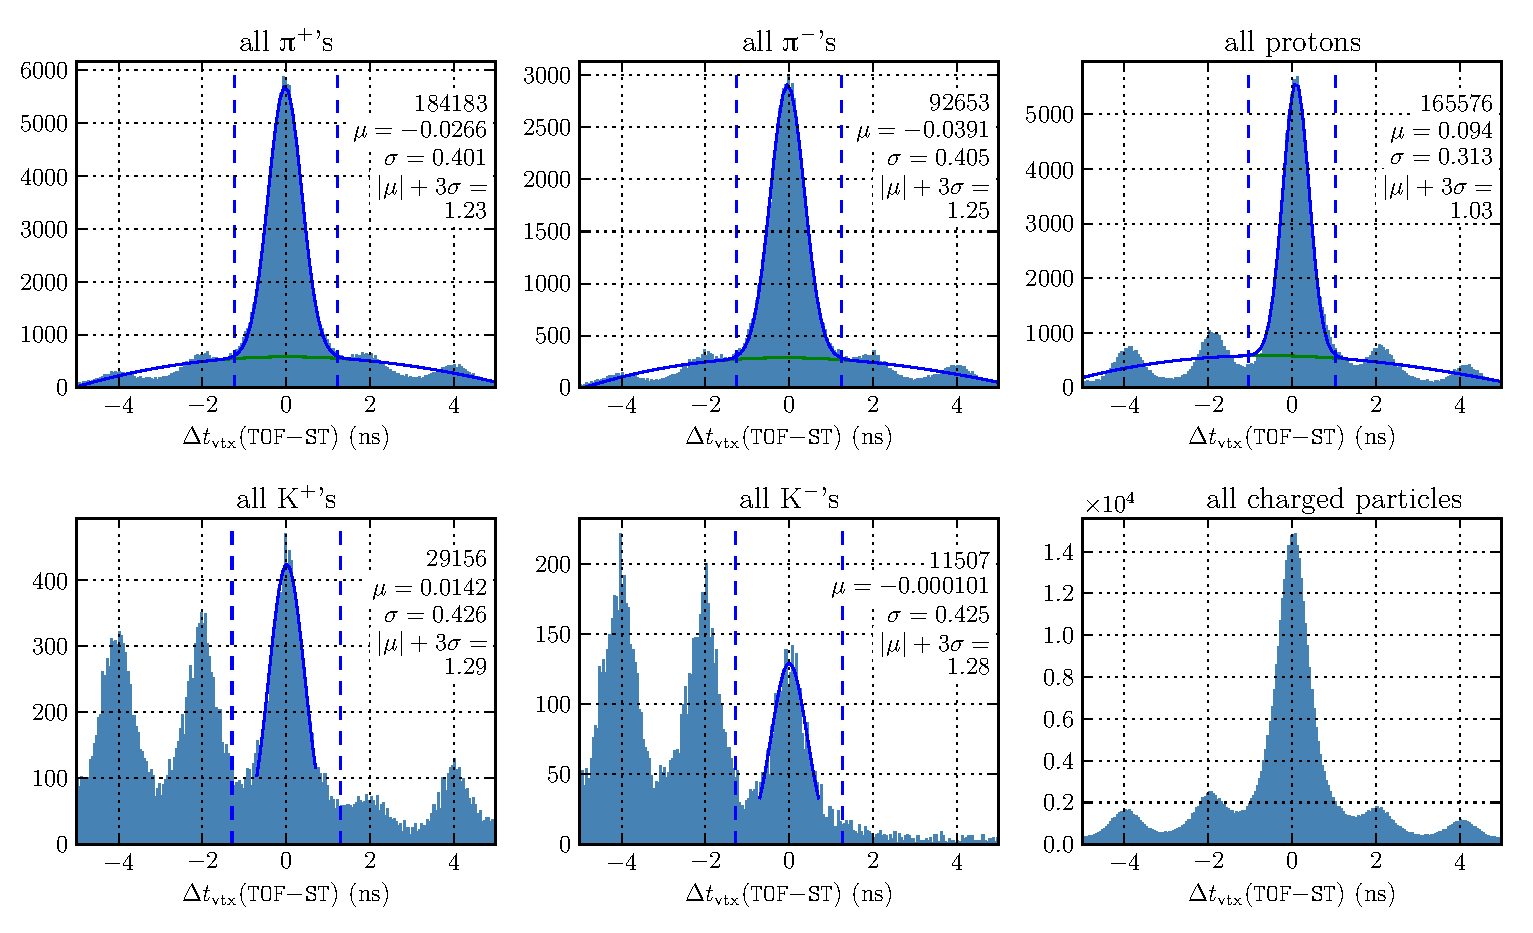
\includegraphics[width=0.9\columnwidth]{figures/calib/st/dvertex_time_st.eps}
\caption[vertex timing, \abbr{TOF-ST}]{\label{fig:dvertex_time_st}Difference in vertex time between that of the photon and of the tracks based on start counter and time-of-flight times. Represents 1.5\% of the total statistics.}
\end{center}\end{figure}


\subsubsection{\label{sec:calib.st.eff}Start Counter Efficiency}

The efficiency of the start counter was calculated by examining the number of tracks with a ST hit after track reconstruction. The ST fired $91.6\%$ of the time, this was calculated from run 57000 since it is a good run and included in production data.

\FloatBarrier

\subsection{\label{sec:calib.dc}Drift Chamber Calibration and Resolution}

\subsubsection{\label{sec:DC.TOF.res}Drift Chamber and TOF smearing parameters in \prog{gpp}}

Tracking in the Drift Chamber of a \abbr{CLAS} Sector is performed using the six superlayers of the \abbr{DC}. A good measure of the the quality of tracking are the \abbr{DC} residuals for each superlayer. After a track is identified using the hit elements in the \abbr{DC} superlayer, It's \abbr{DC} residual is calculated using the TBLA bank as follows:

\begin{verbatim}
fabs(TBLA->tbla[i].fitdoca) - fabs(TBLA->tbla[i].calcdoca)
\end{verbatim}

The values of the DC residuals in the CLAS data are empirically found to be a good fit to a convolution of 2 gaussians - a narrow gaussian and a broad gaussian. During DC calibrations efforts were made to minimize this residual to have maximum reconstruction efficiency. The mean and width of the residuals as a function of superlayer and run number are shown in Figs.~\ref{fig:calib.dc.residuals.mean} and \ref{fig:calib.dc.residuals.wid} respectively.


\begin{figure}\begin{center}
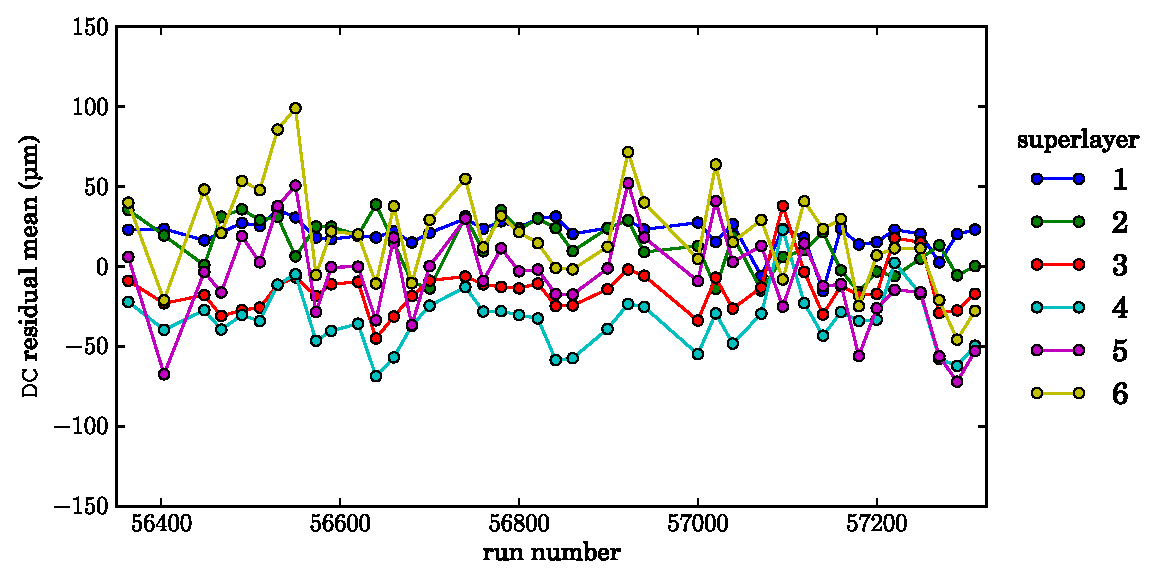
\includegraphics[width=0.6\textwidth]{figures/calib/dc/dc_resid_mean.eps}
\caption[DC Residuals (Mean)]{\label{fig:calib.dc.residuals.mean}Mean of residuals for the drift chambers by superlayer and by run.}
\end{center}\end{figure}

\begin{figure}\begin{center}
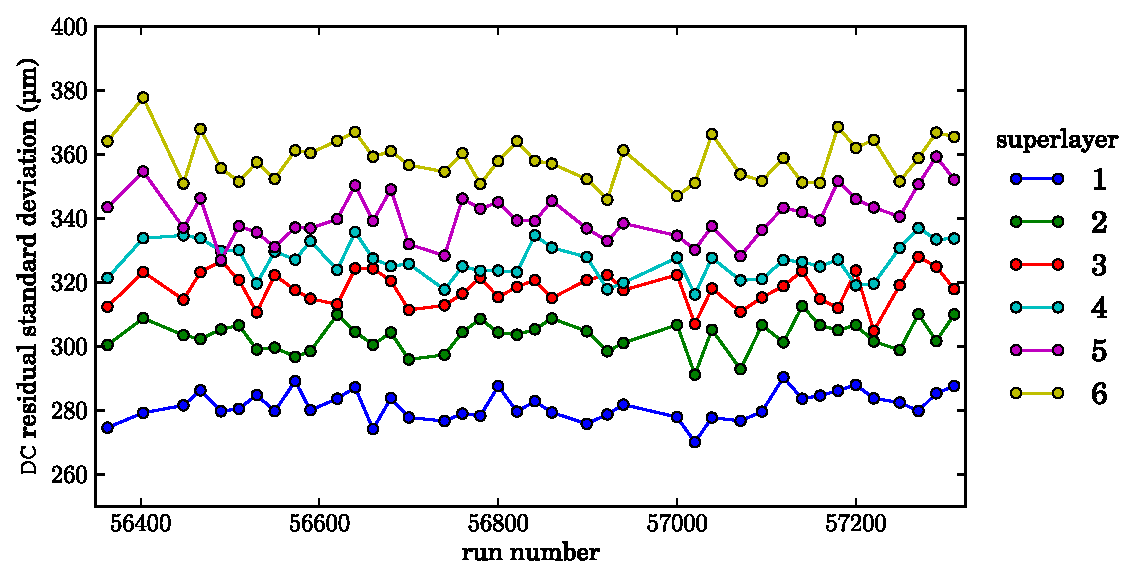
\includegraphics[width=0.6\textwidth]{figures/calib/dc/dc_resid_sigma.eps}
\caption[DC Residuals (Width)]{\label{fig:calib.dc.residuals.wid}Gaussian width of residuals for the drift chambers by superlayer and by run.}
\end{center}\end{figure}

\subsubsection{\label{sec:calib.dc.eff}Drift Chamber Wire Efficiency}
To generate the wiretap for g12, the utility pdu, available in SVN, was used. Maurizio Ungaro made the wiremaps for g12 with the root files [A01 and A02] for each run. These output files are at \url{/home/mukesh/work/pdu_hbook} at Jlab. Root files needed are at \url{/home/mukesh/work/pdu_root}. The values were added to the g12 database. The results of the wiretap are plotted in for each sector:

\begin{verbatim}
http://www.jlab.org/~ungaro/maureepage/proj/dceff/dc_periods/g12.html
\end{verbatim}

\FloatBarrier

\subsection{\label{sec:calib.cc}Cerenkov Calibration and Resolution}

\subsubsection{\label{sec:calib.cc.eff}Cerenkov Efficiency}

\FloatBarrier

\subsection{\label{sec:calib.tof}Time-of-Flight Counter Calibration and Resolution}

\begin{itemize}
    \item The plots shown are for g12's run number 56855, pass0 v7. Did not change to pass1.
    \item Several steps were taken to calibrate the TOF for g12. Listed in C. Bookwalter's dissertation\cite{clas.thesis.bookwalter}:
    \begin{itemize}
        \item Counter status
        \item ADC pedestals
        \item TDC linearization constants
        \item Time-walk corrections
        \item Left-right delay constants
        \item Attenuation length
        \item Minimum-ionizing particle pulse heights
        \item Effective velocity
        \item Paddle-to-paddle offsets
    \end{itemize}
    \item The final time-walk corrections is a mix between constants from g6c and constants derived from g9a laser data using Gamecock.
    \item The plots (Figs.~\ref{plt:tofbetavpneg}--\ref{plt:tofrunbyrun}) included are:
    \begin{itemize}
        \item The TOF velocity ($\beta$) versus momentum by positive and negative tracks.
        \item The RF TOF by paddle ID by sector.
        \item The energy deposited versus momentum by positive and negative tracks.
        \item The TOF mass.
        \item The TOF resolution integrated over all paddles.
        \item The TOF run-by-run performance.
    \end{itemize}
\end{itemize}

\begin{figure}\begin{center}
    \begin{subfigure}{0.5\columnwidth}\begin{center}
        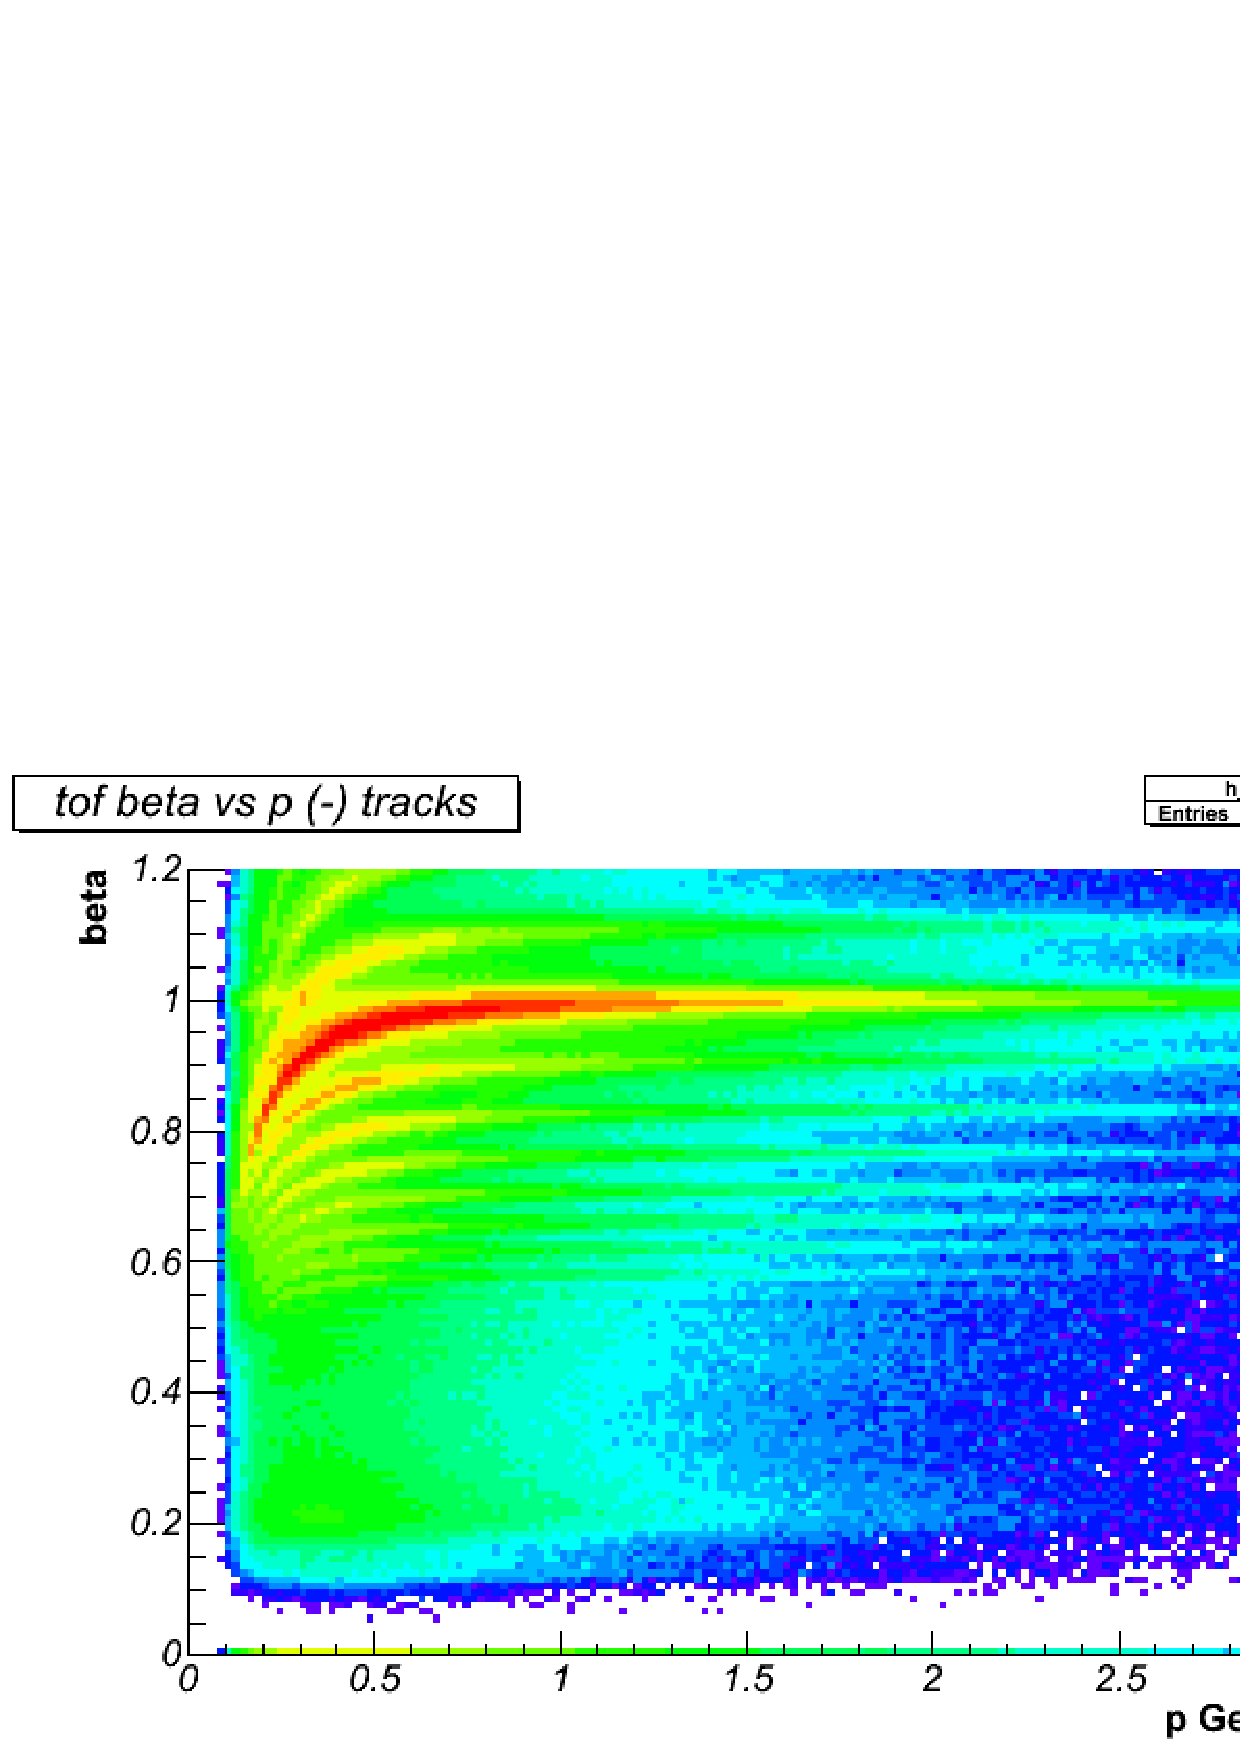
\includegraphics[width=.9\linewidth]{figures/calib/tof/Tof_56855_final_betavpm.pdf}
        \caption{TOF $\beta$ versus momentum for negative tracks}
        \label{plt:tofbetavpneg}
    \end{center}\end{subfigure}\begin{subfigure}{0.5\columnwidth}\begin{center}
        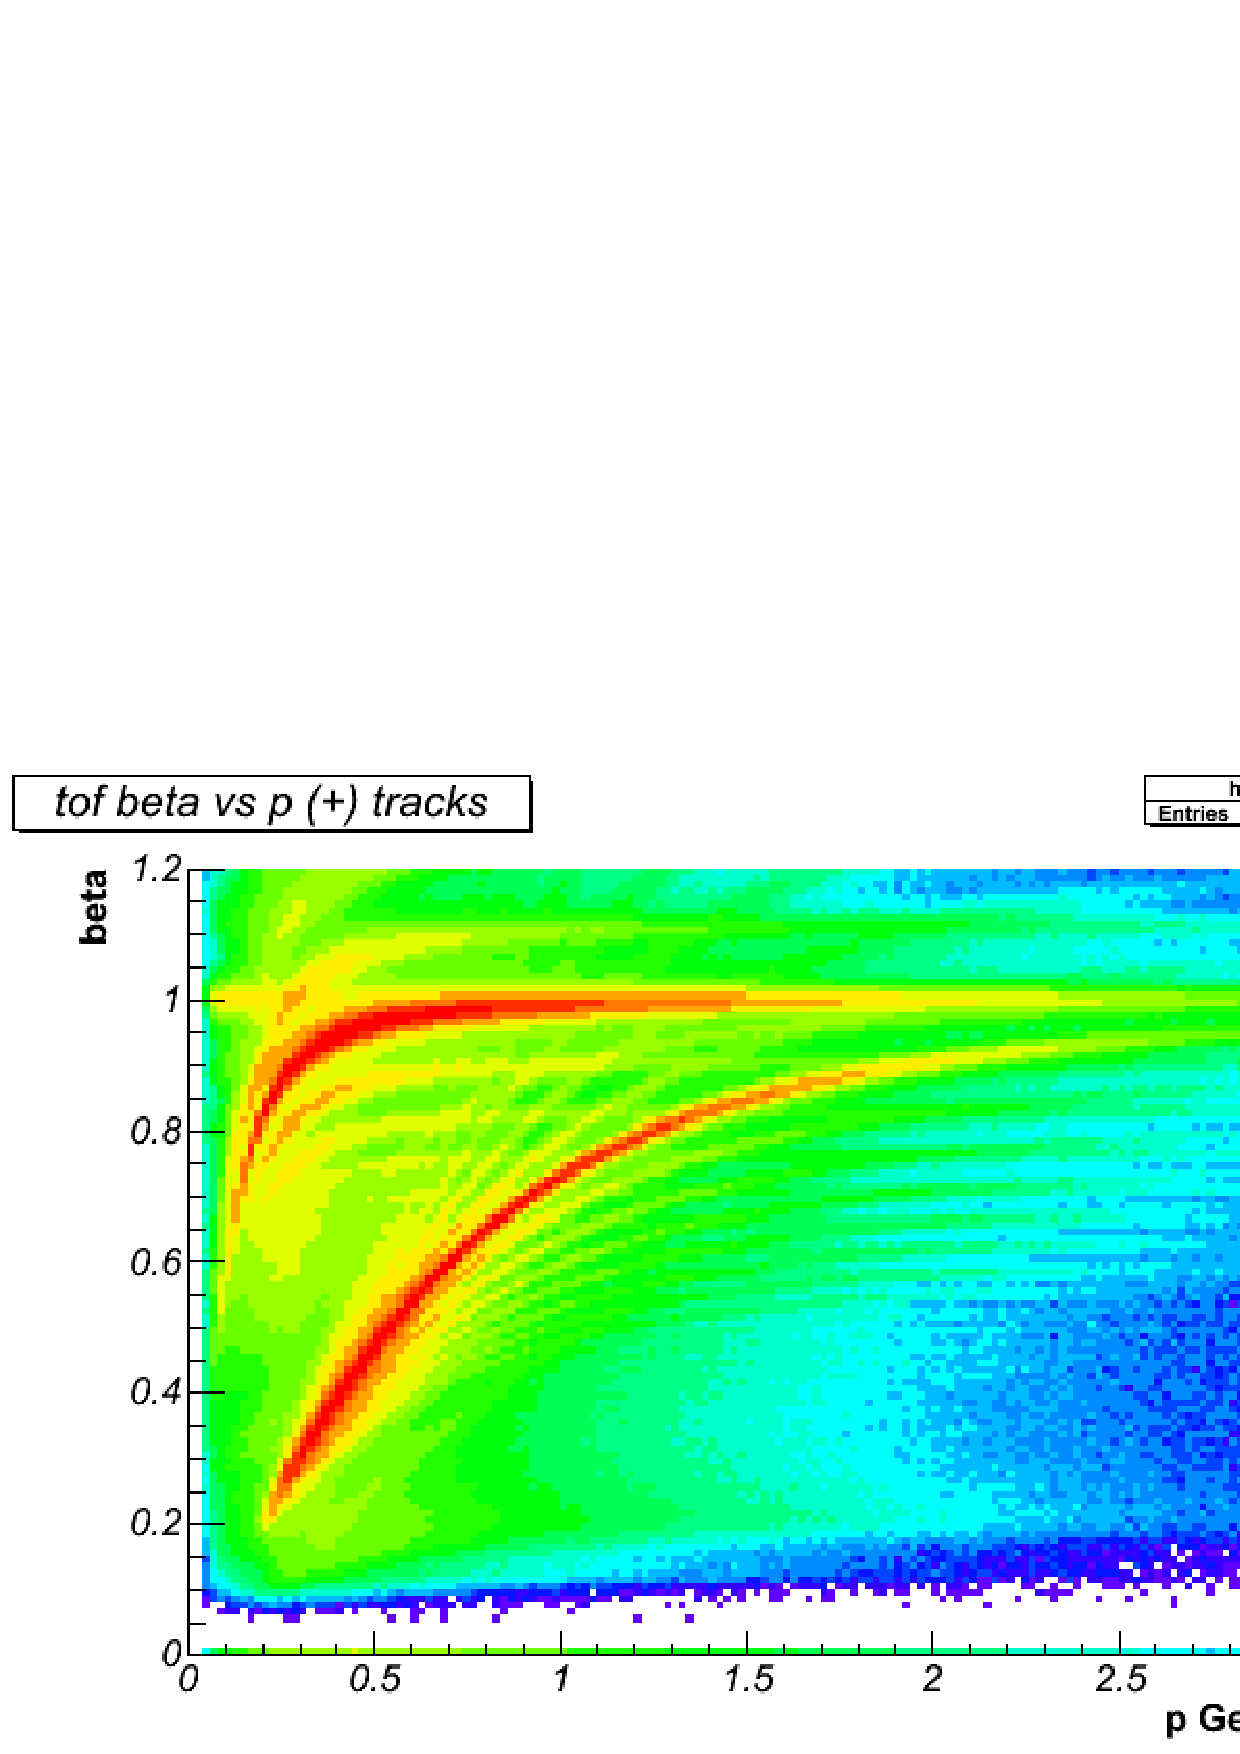
\includegraphics[width=.9\linewidth]{figures/calib/tof/Tof_56855_final_betavpp.pdf}
        \caption{TOF $\beta$ versus momentum for positive tracks}
        \label{plt:tofbetavppos}
    \end{center}\end{subfigure}
\end{center}\end{figure}

\begin{figure}\begin{center}
    \begin{subfigure}{0.5\columnwidth}\begin{center}
        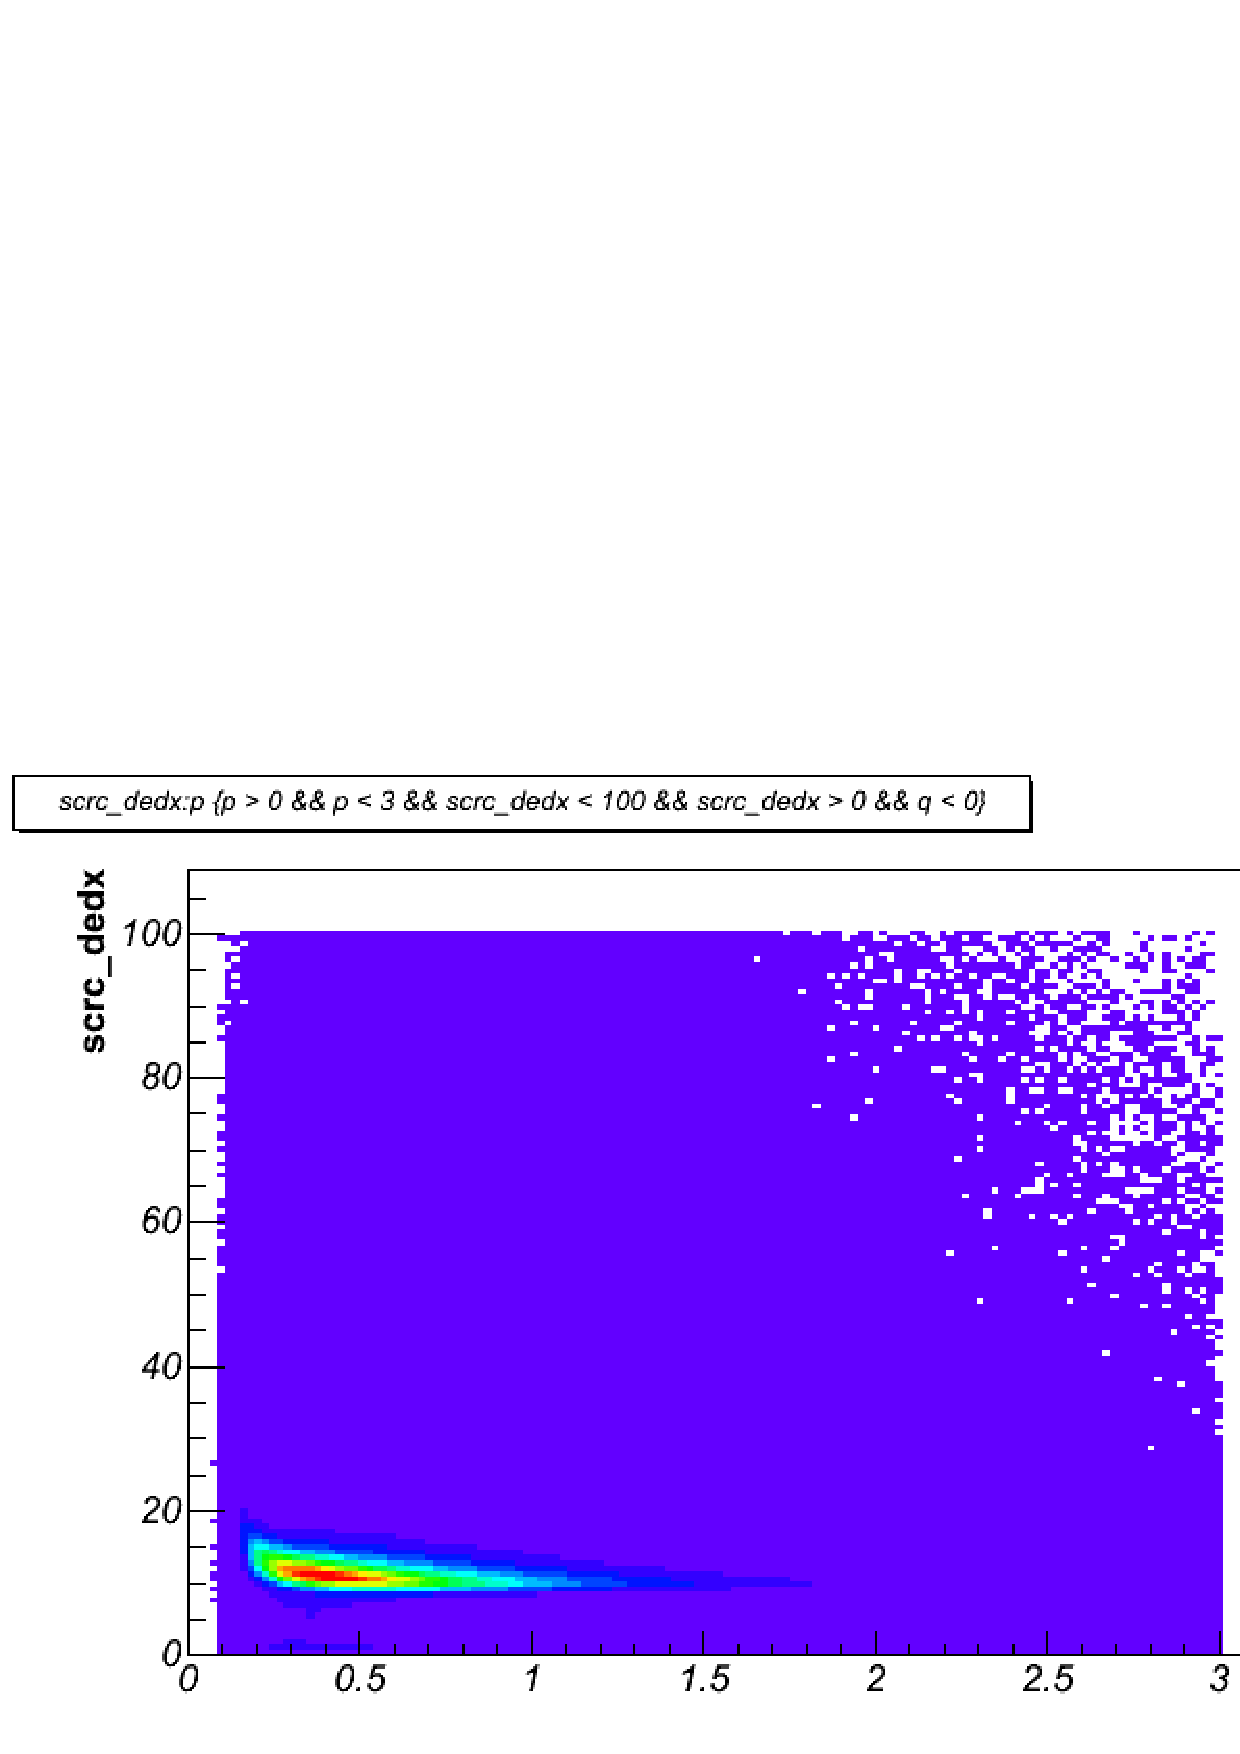
\includegraphics[width=.9\linewidth]{figures/calib/tof/Tof_56855_final_dedxm.pdf}
        \caption{TOF energy deposited versus momentum for negative tracks}
        \label{plt:tofEvpneg}
    \end{center}\end{subfigure}\begin{subfigure}{0.5\columnwidth}\begin{center}
        \includegraphics[width=.9\linewidth]{figures/calib/tof/Tof_56855_final_dedxp.pdf}
        \caption{TOF energy deposited versus momentum for positive tracks}
        \label{plt:tofEvppos}
    \end{center}\end{subfigure}
\end{center}\end{figure}

\begin{figure}\begin{center}
    \begin{subfigure}{0.5\columnwidth}\begin{center}
        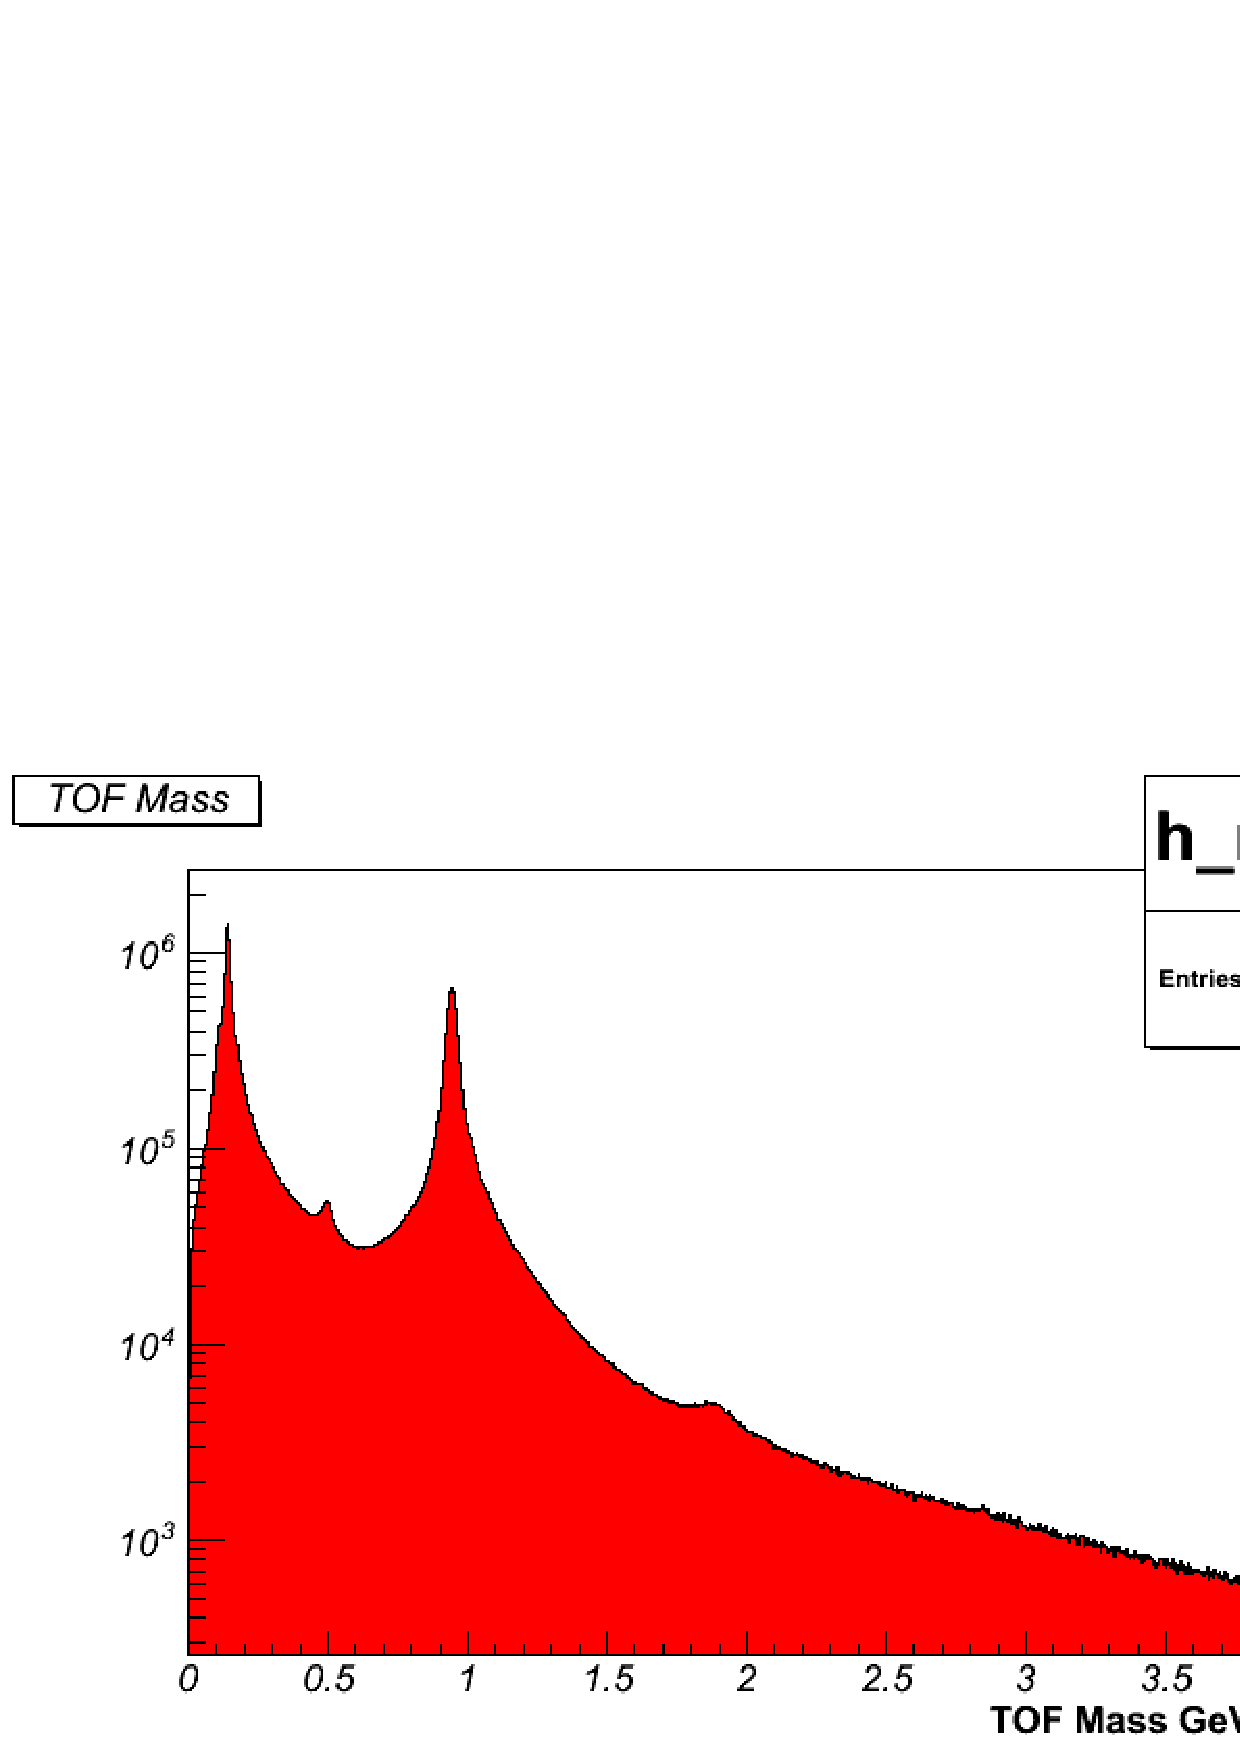
\includegraphics[width=.9\linewidth]{figures/calib/tof/Tof_56855_final_mass.pdf}
        \caption{TOF mass spectrum}
        \label{plt:tofmass}
    \end{center}\end{subfigure}\begin{subfigure}{0.5\columnwidth}\begin{center}
        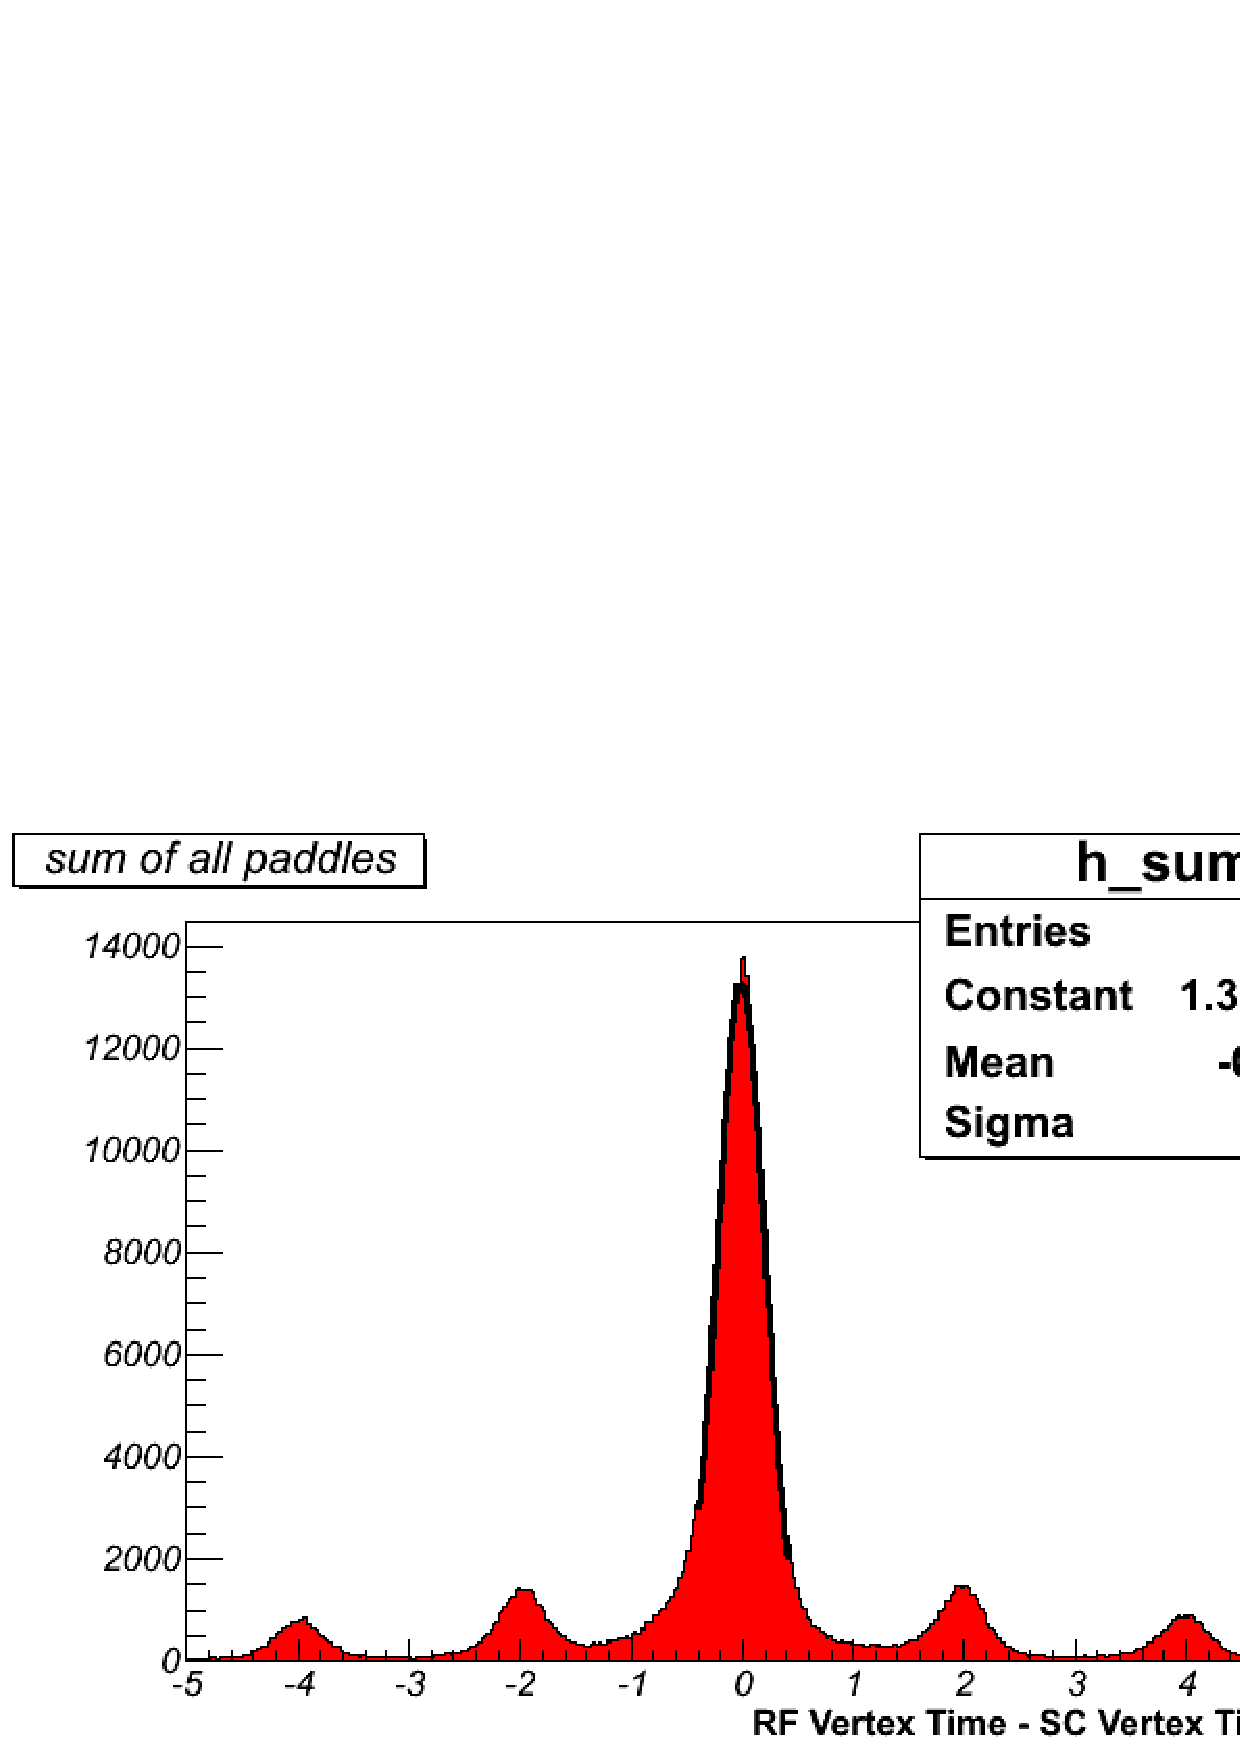
\includegraphics[width=.9\linewidth]{figures/calib/tof/Tof_56855_final_resolution.pdf}
        \caption{TOF resolution integrated over all paddles}
        \label{plt:tofres}
    \end{center}\end{subfigure}
\end{center}\end{figure}

\begin{figure}\begin{center}
    \begin{subfigure}{0.5\columnwidth}\begin{center}
        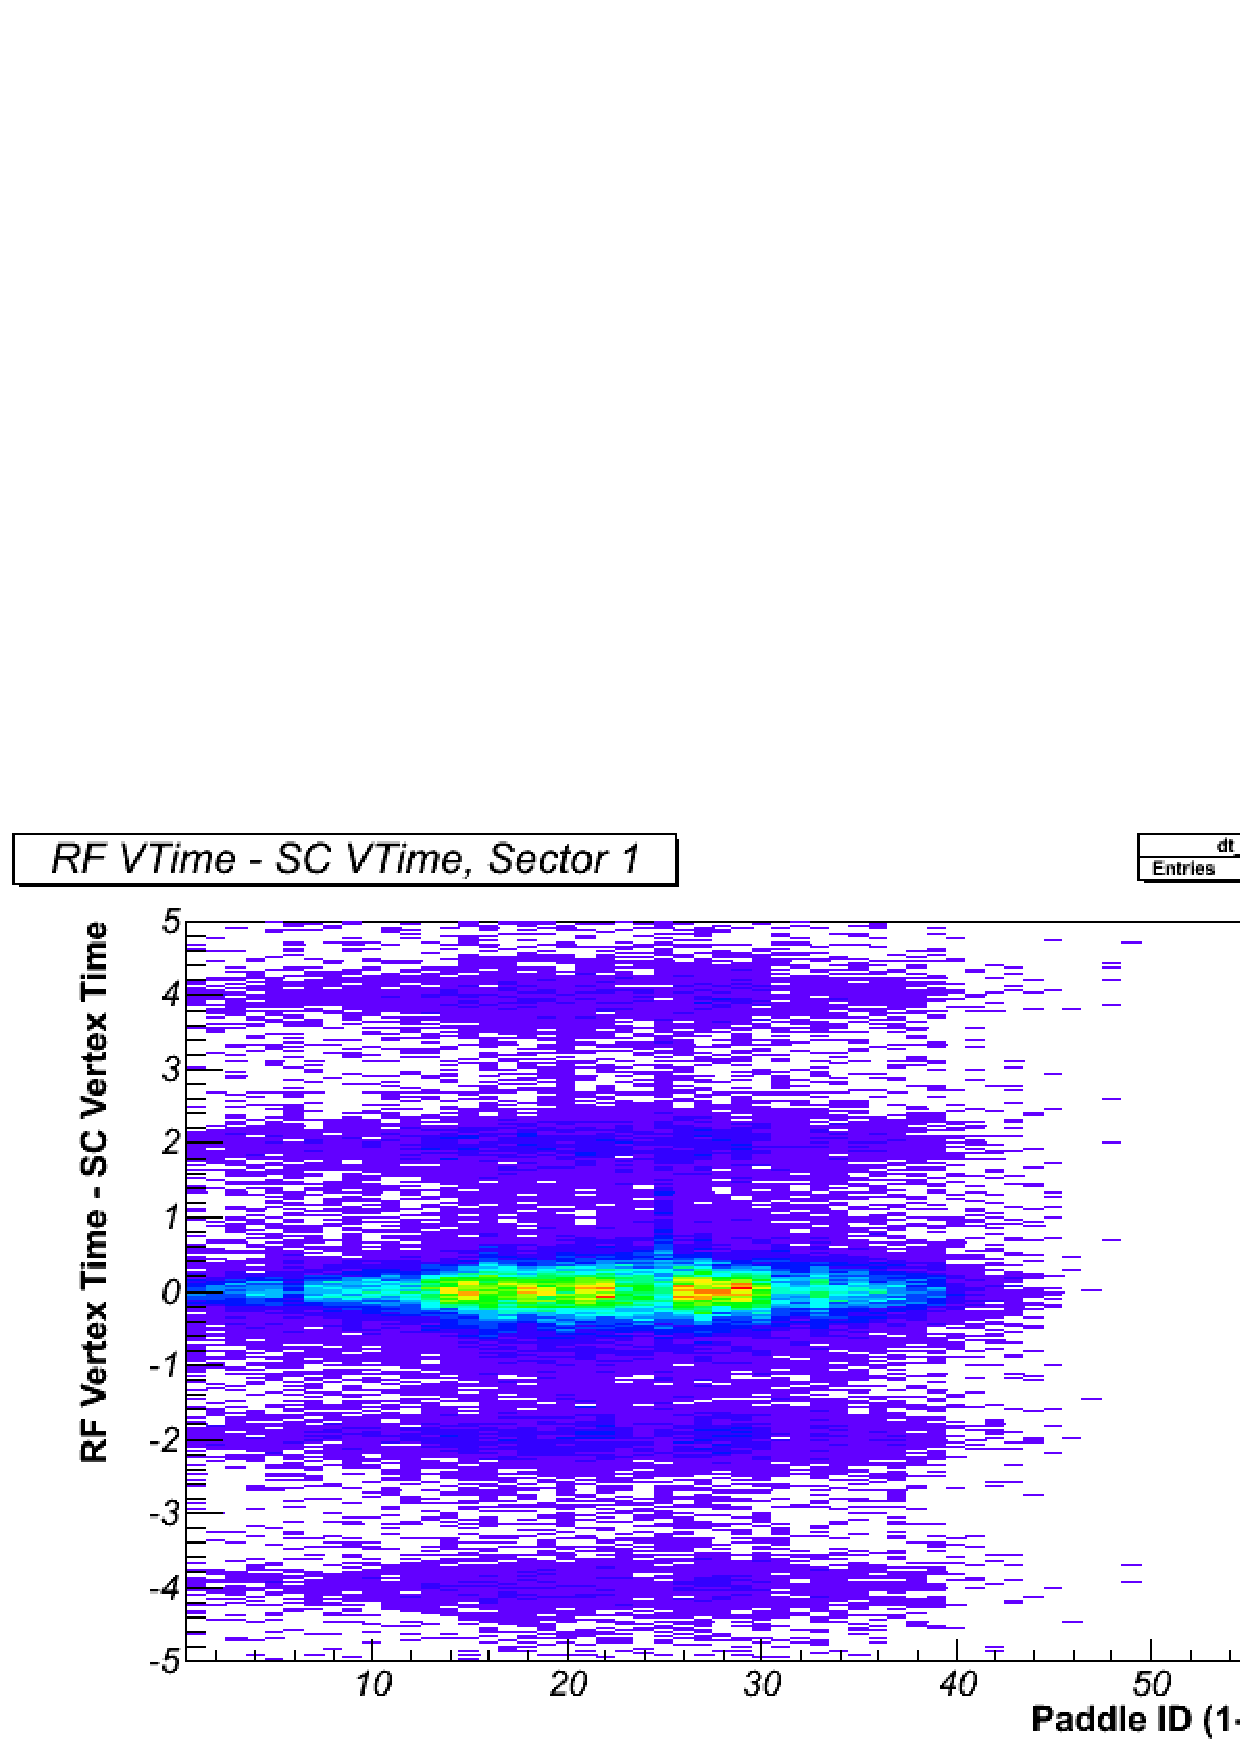
\includegraphics[width=.9\linewidth]{figures/calib/tof/Tof_56855_final_s1p2p.pdf}
        \caption{Representative (sector 1) calibrated timing of the time-of-flight, paddle-by-paddle.}
        \label{plt:tofsec1}
    \end{center}\end{subfigure}\begin{subfigure}{0.5\columnwidth}\begin{center}
        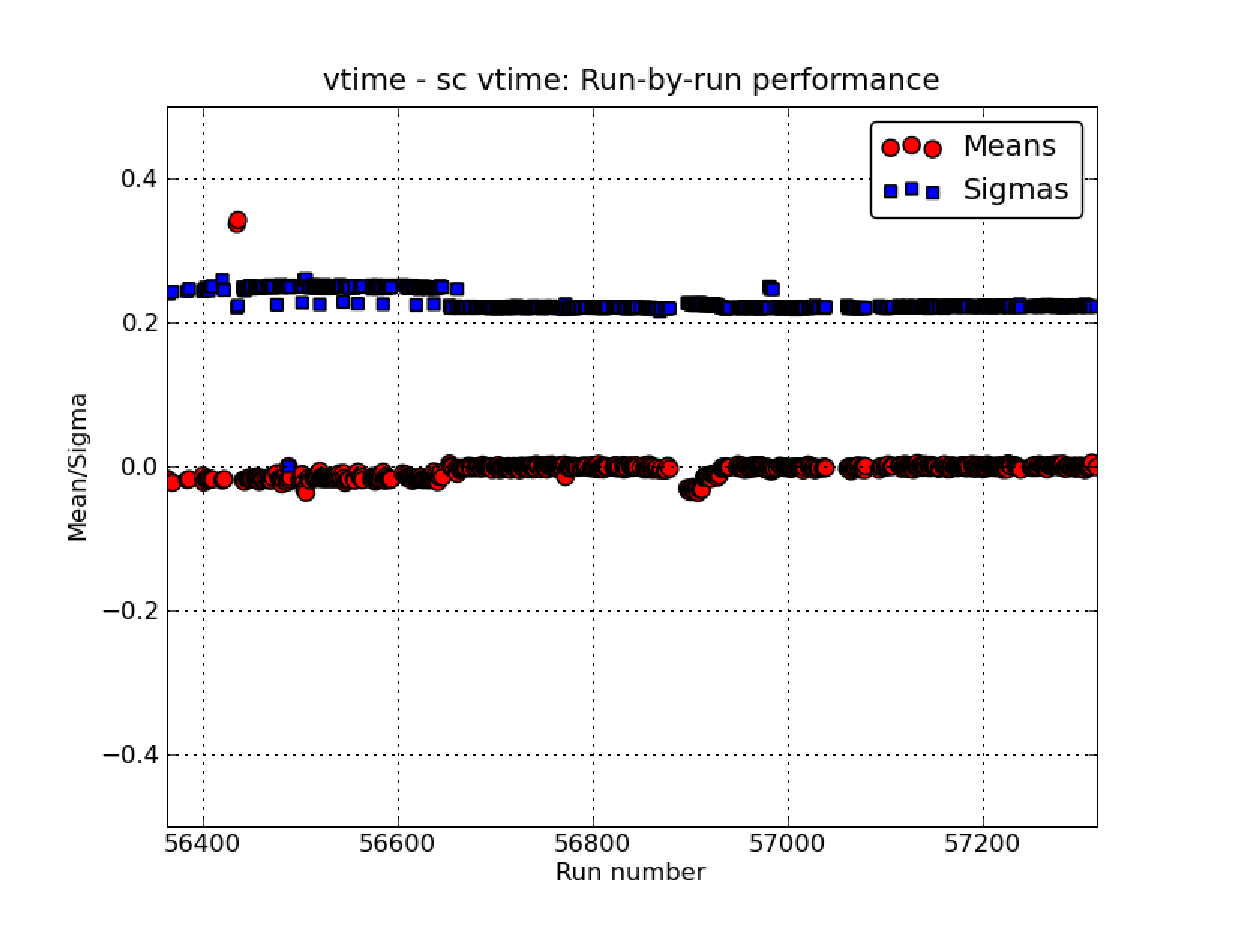
\includegraphics[width=.9\linewidth]{figures/calib/tof/Tof_runscan_p0v7.eps}
        \caption{TOF run-by-run performance}
        \label{plt:tofrunbyrun}
    \end{center}\end{subfigure}
\end{center}\end{figure}

\subsubsection{\label{sec:calib.tof.eff}Time-of-Flight Counter Efficiency and Bad Paddles}

As a standard procedure of the time-of-flight calibrations, the time-of-flight scintillators were initially studied during the calibration period, in which a list~\footnote{Can be obtained using the CLAS calibration database} of scintillators had a faulty ADC or TDC as shown in Table~\ref{tab:craigtof}. Another study, as shown below, was conducted to determine the efficiency of each paddle and to reevaluate the status of their ADC and TDC. Due to the more stringent requirements of paddle efficiency in the study below, more paddles were considered to be faulty than in the initial study. Table~\ref{tab:diff} shows the additional paddles which were considered to be inefficient.

\begin{table}
\begin{minipage}{\textwidth}
\begin{center}
\begin{singlespacing}

\caption{\label{tab:craigtof}List of faulty paddles as compiled during calibration}
    
\begin{tabular}{llp{.43\textwidth}}

\hline \hline

Sector & SCID & Notes \\

\hline

1 & 6 & No ADCR and TDCR \\
2 & 8 & No ADCL and TDCL \\
2 & 34 & No ADCL and TDCL \\
3 & 11 & No ADCR and TDCR \\
3 & 57 & No ADCL, ADCR, TDCL, and TDCR \\
4 & 48 & No ADCL and TDCL \\
5 & 57 & No ADCL, ADCR, TDCL, and TDCR \\
6 & 5 & No ADCR and TDCR \\

\hline \hline

\end{tabular}

\end{singlespacing}
\end{center}
\end{minipage}
\end{table}
 % label: tab:craigtof

\begin{figure}\begin{center}
    \includegraphics[trim=0 40 10 40,clip,width=.40\linewidth]{figures/calib/tof/tofko/occp.eps}
    \caption{Relative occupancy of all scintillators}
    \label{plt:occp}
\end{center}\end{figure}

To determine efficiency of each scintillator paddle, the number of hits~\footnote{The data used were obtained from the \texttt{clas\underline{\hspace{5pt}}0$[$run\#$]$.A01} files located in \texttt{$/$mss$/$clas$/$g12$/$data$/$}} registered by every paddle was recorded~\footnote{This was done by using \texttt{bosdump -GSC} and parsing its output}. The relative occupancy of paddle $i$ in sector $j$ is defined the following way: list the number of hits recorded by all paddle $i$'s in sectors $\neq j$ and remove the ones with the most and least hits from the list. Take the average number of hits of the remaining three paddles. The relative occupancy is defined as
\[
100 \times \frac{ \mathrm{Number of hits in paddle } i \mathrm{ of sector } j}{\mathrm{Average of remaining three paddles}} \hspace{2pt}\%
\]

Fig.~\ref{plt:occp} shows the relative occupancy of all scintillators plotted on a single histogram. A paddle is defined as inefficient if it is greater than two standard deviations below the mean relative occupancy of all scintillators. Table.~\ref{tab:occp} shows the paddles which are below two (left) or three (right) standard deviations below the mean relative occupancy.

\begin{table}
\begin{minipage}{\textwidth}
\begin{center}
\begin{singlespacing}

\caption{\label{tab:occp}Paddles below two and three standard deviations from the mean relative occupancy}

\begin{tabular}{lcc}

\hline \hline

 &  $2 \sigma = 92.49\%$ &  $3 \sigma = 89.05\%$ \\
 
\hline

Sector 1 & 35 (91.20\%) & 40 (87.87\%), 41 (82.63\%), 56 (83.37\%) \\
Sector 2 & 2 (92.38\%), 35 (90.11\%), 50 (91.99\%) &  41 (87.31\%), 56 (87.98\%)\\
Sector 3 & 35 (90.59\%) & 40 (88.98\%), 41 (83.29\%)\\
Sector 4 &  & 41 (83.61\%) \\

\hline \hline

\end{tabular}

\end{singlespacing}
\end{center}
\end{minipage}
\end{table}
 % label: tab:occp

\subsubsection{\label{sec:calib.tof.adctdc}ADC and TDC Values}

\begin{figure}\begin{center}
    \includegraphics[width=0.70\linewidth]{figures/calib/tof/tofko/adctdcval.eps}
    \caption{\label{plt:adctdcval}Top: ADC values of all scintillators. Left ADC (ADCL) values are on the left and right ADC values are on the right (ADCR). Shaded in red are events recorded with an ADC value of zero or maximum. Bottom: Same as Top but for TDC values}
\end{center}\end{figure}

The occupancy alone is not enough to determine which scintillators are bad. The ADC and TDC values for all scintillators were also recorded and studied. Fig.~\ref{plt:adctdcval} shows the ADC and TDC values for all scintillators. Some of the events registered had an ADC or TDC value of zero or a maximum ADC value (shaded in red). The percentage of events a scintillator recorded either a TDC or ADC value of zero or maximum ADC value was studied as shown in Figs.~\ref{plt:adc0vSCID}, \ref{plt:adcMvSCID} and \ref{plt:tdc0vSCID}. Figures~\ref{plt:adc0vSCID}, \ref{plt:tdc0vSCID} and \ref{plt:proj} assisted in determining bad paddles. It (is to be) was decided that a paddle cannot have more than $50\%$ of its ADC (left or right) values be equal to zero or more than $45\%$ of its TDC (left or right) values equal to zero. Table~\ref{tab:adctdc0} shows which paddles fall in these categories. Table~\ref{tab:tofko} shows which scintillators should be knocked out due to low occupancy or too many null ADC or TDC values. Due to the small number of events in which a maximum ADC value is obtained, it is not recommended in knocking paddles out based on this measure. However, Table~\ref{tab:adcM} shows the paddles which attain a maximum ADC value on more than $2.5\%$ of its registered events.

\begin{table}
\begin{minipage}{\textwidth}
\begin{center}
\begin{singlespacing}

\caption{\label{tab:adctdc0}Paddles which registered an ADC or TDC value of zero greater than 50\% and 45\%, respectively, of its entries}

\begin{tabular}{lp{.43\textwidth}p{.43\textwidth}}

\hline \hline

 &  \% Events with ADCL or ADCR = 0 \( > \) 50\% &  \% Event with TDCL or TDCR = 0 \( > \) 45\% \\
 
\hline

Sector 1 & 6 (100\% ADCR) & 6 (100\% TDCR), 46 (97.89\% TDCL), 50 (98.11\% TDCL) \\
Sector 2 & 8 (100\% ADCL), 34 (100\% ADCL), 44 (50.22\% ADCL), 54 (52.00\% ADCR) &  8 (100\% TDCL), 34 (100\% TDCL), 44 (47.51\% TDCL), 54 (47.10\% TDCR)\\
Sector 3 & 11 (100\% ADCR), 56 (74.75\% ADCR) & 11 (100\% TDCR), 56 (62.79\% TDCR)\\
Sector 4 & 48 (100\% ADCL) & 48 (100\% TDCL) \\
Sector 5 & 48 (77.98\% ADCL) & 48 (76.10\% TDCL)\\
Sector 6 & 5 (100\% ADCR), 56 (59.30\% ADCR) & 1 (98.78\% TDCL), 5 (100\% TDCR), 33 (97.78\% TDCL) \\

\hline \hline

\end{tabular}

\end{singlespacing}
\end{center}
\end{minipage}
\end{table}
 % label: tab:adctdc0

\begin{table}
\begin{minipage}{\textwidth}
\begin{center}
\begin{singlespacing}

\caption{\label{tab:tofko}Union of \ref{tab:occp,tab:adctdc0} (Recommended list of paddles to knockout)}

\begin{tabular}{lc}

\hline \hline

Sector 1: & 6, 35, 40, 41, 50, 56\\
Sector 2: & 2, 8, 34, 35, 41, 44, 50, 54, 56\\
Sector 3: & 11, 35, 40, 41, 56\\
Sector 4: & 41, 48 \\
Sector 5: & 48\\
Sector 6: & 1, 5, 33, 56 \\

\hline \hline

\end{tabular}

\end{singlespacing}
\end{center}
\end{minipage}
\end{table}

 % label: tab:tofko

\begin{table}
\begin{minipage}{\textwidth}
\begin{center}
\begin{singlespacing}

\caption{\label{tab:diff}Paddles in \ref{tab:tofko} not included in \ref{tab:craigtof}}

\begin{tabular}{lc}

\hline \hline

Sector 1: & 35, 40, 41, 50, 56 \\
Sector 2: & 2, 35, 41, 44, 50, 54, 56 \\
Sector 3: & 35, 40, 41, 56 \\
Sector 4: & 41 \\
Sector 5: & 48 \\
Sector 6: & 1, 33, 56 \\

\hline \hline

\end{tabular}

\end{singlespacing}
\end{center}
\end{minipage}
\end{table}
 % label: tab:diff

\begin{table}
\begin{minipage}{\textwidth}
\begin{center}
\begin{singlespacing}

\caption{\label{tab:adcM}Paddles with percentage of hits registering a maximum ADC value \( > \) 2.5\% of its events}

\begin{tabular}{lc}

\hline \hline

Sector 1: & 20 (2.93\% ADCL) \\
Sector 3: & 20 (4.26\% ADCL) \\

\hline \hline

\end{tabular}

\end{singlespacing}
\end{center}
\end{minipage}
\end{table}

 % label: tab:adcM

\begin{figure}\begin{center}
    \includegraphics[width=0.75\textwidth]{figures/calib/tof/tofko/adc.eps}
    \caption{\label{plt:adc0vSCID}Percentage of hits registering an ADC value of 0 for all scintillators. Left ADC (ADCL) are on the left and right ADC (ADCR) values are on the right}
\end{center}\end{figure}

\begin{figure}\begin{center}
    \includegraphics[width=0.75\textwidth]{figures/calib/tof/tofko/tdc.eps}
    \caption{\label{plt:tdc0vSCID}Percentage of hits registering an TDC value of 0 for all scintillators. Left TDC (TDCL) are on the left and right TDC (TDCR) values are on the right}
\end{center}\end{figure}

\begin{figure}\begin{center}
    \includegraphics[width=0.75\textwidth]{figures/calib/tof/tofko/adcMax.eps}
    \caption{\label{plt:adcMvSCID}Percentage of hits registering a maximum ADC value for all scintillators. Left ADC (ADCL) are on the left and right ADC (ADCR) values are on the right}
\end{center}\end{figure}

\begin{figure}\begin{center}
    \includegraphics[width=0.8\textwidth]{figures/calib/tof/tofko/adctdc0perc.eps}
    \caption{\label{plt:proj}Top: Y axis projections of Fig.~\ref{plt:adc0vSCID}. Bottom: Y axis projections of Fig.~\ref{plt:tdc0vSCID}}
\end{center}\end{figure}

\begin{v2}
\subsubsection{\label{sec:calib.tof.resolution}Time-of-Flight Paddle Resolution}
So far, the selection of bad paddles is based only the raw data, which is only good for the initial selection. We further investigate the timing resolution of each paddle by run in order to determine stability of their resolutions throughout the experiment. The following data analyzed were from events containing $p \pi^{+} \pi^{-}$ in the final state. For the $\pi^{+}$ and $\pi^{-}$, the difference between the measured time-of-flight and the expected time-of-flight for a given run was plotted and fitted to a Gaussian. This was done for every paddle and every run. We define the resolution of that paddle to be the standard deviation of the fit. 
%Figure~\ref{plot:example.tofresVrun} shows an example of this. The TOF resolution for every paddle as a function of run number is stored in the g12 wiki page. 
A few paddles that had not been previously knocked out had drifts on either the resolution or the mean $\Delta$ TOF and were not properly calibrated. Table~\ref{tab:tofko.additional} shows which paddles should ideally be knocked out due to this. However, the track dependent efficiency correction was derived without these paddles being knocked out. Consequently, the these paddles should not be knocked out if using the track dependent efficiency correction. If one would like to use these additional time-of-flight knockouts, then one would need to re-derive the track dependent efficiency corrections. Figure~\ref{plot:example.goodpaddle} shows an example of a good paddle's resolution and mean $\Delta$ TOF while figure~\ref{plot:example.badpaddle} shows and example of a bad paddle. The TOF resolution for every paddle by run is stored in the g12 wiki.


\begin{figure}\begin{center}
      \includegraphics[width=0.95\columnwidth]{figures/calib/tof/goodexample.pdf}
   \caption{\label{plot:example.goodpaddle}TOF resolution as a function of run number for a good paddle}
\end{center}\end{figure}

\begin{figure}\begin{center}
      \includegraphics[width=0.95\columnwidth]{figures/calib/tof/badexample.pdf}
   \caption{\label{plot:example.badpaddle}TOF resolution as a function of run number for a bad paddle}
\end{center}\end{figure}
\end{v2}

\FloatBarrier

\subsection{\label{sec:calib.ec}Electrocalorimeter Calibration and Resolution}

\subsubsection{\label{sec:calib.ec.eff}Electrocalorimeter Efficiency and Bad Paddles}

\FloatBarrier


\section{\label{sec:data}Procedure for Data Analysis}


The broad steps for analysis of a specific reaction in the \desg{g12} data are:
\begin{enumerate}
    \item determine event selection cuts to be used on a small subset of the data,
    \item skim the ``cooked'' data and produce an ntuple which will include the four-momenta and a few other parameters needed for the final analysis,
    \item tune the analysis on the data to get the final yields,
    \item run simulations through the tracker/digitizer (\prog{gsim}), smearing (\prog{gpp}), track reconstruction (\prog{a1c}), and the final analysis programs to obtain efficiencies and acceptances,
    \item calculate the beam flux corresponding to the data analyzed,
    \item tie the yields, acceptances and flux together to come up with a final answer and an absolute scaling.
\end{enumerate}
One or more of these steps, or parts of these steps, may not be necessary for a given analysis and they do not have to be done this order. This section discusses where to find the various programs and files needed for each of these steps.

\subsection{\label{sec:data.cook}``Pass1'' Cooking and Data Reconstruction}

This section describes the process of reconstructing the raw data into almost-physics-ready form. Broadly speaking, the output of this procedure is the three-momenta of the detected final-state particles and various supporting measurements such as timing or energy deposit which is used for particle identification.

The reconstruction program \texttt{a1c} requires an environment variable to point to the correct run index for this run period. This can be set in a bash shell using the command:
\begin{verbatim}
export CLAS_CALDB_RUNINDEX=calib_user.RunIndexg12
\end{verbatim}
The command to cook the gsim bos file using the \texttt{a1c} program is:
\begin{verbatim}
a1c -T4 -sa -ct1930 -cm0 -cp0 -X0 -d1 -F -P0x1bff -z0,0,-90 \
  -Aprlink_tg-90pm30.bos -o3pi.a1c 3pi.gpp
\end{verbatim}
which will produce BOS files similar to the ``cooked'' data. This is the same command to be used to \emph{recook} raw data files. The options shown here will be slightly different for simulated data since \desg{CLAS} does not treat simulation in exactly the same way as real data. This is a legacy issue that has been well documented in previous experiments and we will merely say that one will have to add the option ``\verb+-X0+'' when running the \prog{a1c} reconstruction program. This is mentioned again in Sec.~\ref{sec:sim.recon} where we discuss the reconstruction of simulated data.

There was only one ``physics'' pass of the \desg{g12} data, labeled \texttt{pass1}, which represents 99\% of the reconstructable data taken. It was determined that tracking down that last 1\% was not worth the effort. On JLab's common user environment (\texttt{CUE}), the cooked data can be found here:
\begin{center}
    \texttt{/mss/clas/g12/production/pass1/bos}
\end{center}
and the raw data can be found here:
\begin{center}
    \texttt{/mss/clas/g12/data/}
\end{center}
Please see JLab's SciComp help pages on how to get these files off the mass storage system. The source code for pass1 was consistent with revision 4715 in the Subversion repository found here:
\begin{center}
    \url{https://jlabsvn.jlab.org/svnroot/clas/trunk}
\end{center}
which was linked against the 2005 version of the \prog{CERNLIB}.

\FloatBarrier





\subsection{\label{sec:data.pass1}Obtaining Reconstructed Data}

All reconstructed data resides in BOS files on the tape-silo at JLab under the directory:
\begin{align}
\texttt{/mss/clas/g12/production/pass1/bos} \nonumber
\end{align}
which contains the following subdirectories or ``categories'' used for event-sorting:
\begin{description}
    \item[1-1ckaon1ctrk] Events which have at least 2 charged tracks, one of which is a ``possible kaon.'' A possible kaon is either a track that the \abbr{PART} bank says is a kaon, or a high-momentum charged pion ($> 2.0$~GeV), or a really high momentum proton ($> 3.0$~GeV). The idea of this selection is to leave no kaon behind.
    \item[2-2pos1neg\_not\_1ckaon1ctrk] Two-positive and one-negative ($++-$) inclusive events which are \emph{not} included in \emph{1-1ckaon1ctrk}. So, for example, if you wanted all ($++-$) events you would have to use both this category and \emph{1-1ckaon1ctrk}.
    \item[3-2ctrk\_not\_2pos1neg\_1ckaon1ctrk] Events with 2 or more charged tracks which do not qualify for either \emph{1-1ckaon1ctrk} or \emph{2-2pos1neg\_not\_1ckaon1ctrk}.
    \item[4-not\_2ctrk\_2pos1neg\_1ckaon1ctrk] Physics events that do not fit into categories 1, 2, or 3.
    \item[5-other] Non-physics events which may include scalers and such.
    \item[6-1lepton] Redundant set of all events with a single ``possible lepton'' according to the
    \begin{align}
        \texttt{ClasParticle::isMaybeLepton()} \nonumber
    \end{align}
    method in the ClasEvent analysis suite.
    \item[7-4ctrk] Redundant set of all four-charged track events.
    \item[8-ppbar] Redundant set of all proton, anti-proton events according to the PART bank.
\end{description}
Note that the first five of these categories are \emph{mutually exclusive and complete} while the last three are completely redundant and are provided for convenience. Non-physics events are included in the fifth (``other'') skim. If one wishes to synchronize these events with their data, they have some options. Perhaps the easiest is to process the raw data which is completely ordered. Timestamps could be used instead, provided they exist in the non-physics skim.

\paragraph{This bears repeating since it is a non-standard sorting of the cooked data:} The five categories numbered 1 through 5 listed above consist of one and only one of \emph{every} event recorded by the data acquisition during the g12 run period for the set of run which were deemed ``good.'' A specific single event will only be found in one of the first five categories. If you want to run on events that are described by category number 4 for example, you will have to include the data in categories 1 through 3 since these will also satisfy category 4 by design and by definition.


The total size of the reconstructed data is 211~TiB consisting of 26.2 billion triggers. The secondary skims (6--8) total 31~TiB. The breakdown of the size of the skims is shown in Table~\ref{tab:skimsize}.

\begin{table}[htpb]
\begin{center}

\begin{minipage}{0.8\textwidth}

\caption{\label{tab:skimsize}Size of skims both in data-size and number of events.}
\begin{center}
\begin{tabular}{ccl}

\hline \hline

size (TiB) & events (G) & skim \\

\hline

50 & 6.2 & 1-1ckaon1ctrk \\
31 & 3.8 & 2-2pos1neg\_not\_1ckaon1ctrk \\
68 & 8.4 & 3-2ctrk\_not\_2pos1neg\_1ckaon1ctrk \\
62 & 7.7 & 4-not\_2ctrk\_2pos1neg\_1ckaon1ctrk \\
0.26 & 0.033 & 5-other \\

\hline

17 & 2.1 & 6-1lepton \\
13 & 1.6 & 7-4ctrk \\
1 & 0.124 & 8-ppbar \\

\hline \hline

\end{tabular}
\end{center}

\end{minipage}

\end{center}
\end{table}
 % tab:skimsize


Typical analyses with \desg{g12} will start with the particles as identified in the \abbr{PART} bank as default in the \prog{ClasEvent} analysis suite. This provides the basic four-momenta of the tracks and their identification which is based on mass calculated from the time-of-flight. The photon associated with the event is then taken from the \abbr{TAGR} bank and the one closest in-time with the tracks is usually taken.

For a deeper analysis, one can get information for specific hits in a given subsystem by following the pointers in the \abbr{PART} and \abbr{TBID} bank to the \abbr{TBTR}, \abbr{SCRC}, \abbr{ECHB} or other similar banks. Most of the relevant banks needed for this type of investigation are included in the cooked data though several raw banks were dropped to save space. To recover the missing banks one would have to go back to the raw data and recook using the \prog{a1c} program though we anticipate this will be a rare event.


The following banks were written out to tape in the pass1 reconstructed data: \abbr{CC CC01 CCPB CCRC CL01 DCPB DSTC EC EC1 EC1R ECHB ECPB ECPC ECPI ECS EPIC EVNT FBPM HBER HBID HBTR HEAD HEVT HLS LCPB MVRT PART RGLK S1ST SC SC1 SCPB SCR SCRC SCS ST1 STN0 STN1 STPB STR STSN SYNC TAGE TAGI TAGR TBER TBID TBTR TDPL TGBI TGPB TGS TRGS TRKS TRL1}. Note that the SEB-related banks (\abbr{EVNT} etc.) were written out. These may be used for any analysis though care should be taken not to mix these with the \abbr{PART}-related series of banks except where there is an apparent redundancy.


\subsection{\label{sec:corrections}\desg{g12}-Specific Corrections}

\subsubsection{\label{sec:corrections.pcor}Final-State Particle Momentum Corrections}

The event reconstruction of a particle track in CLAS starts in region 1 of the DC after the track has gone through the target and start counter. To reconstruct the track back to the event vertex, additional energy loss from the target and start counter are included. The standard CLAS ELOSS package provides the required functionality as detailed in Ref. \cite{eloss}. ELOSS corrects for the energy lost as charged tracks go from the event vertex through the beam pipe, target, and start counter using the Bethe-Bloch equation \cite{pdg} to relate the material characteristics and path length to energy loss.

The momenta of the tracks as measured by the Drift-Chamber (\texttt{DC}) have a systematic shift within each sector as a function of azimuthal-angle $\phi$ of one of the tracks. This can be seen in the ``tranverse momentum balance'' plots shown in Fig.~\ref{fig:pbal.before}. The transverse momentum balance for a given particle is defined as the sum of the momentum of the other particles projected onto the line that is perpendicular to the beam having the same $\phi$ angle as the given particle minus its momentum transverse to the beam.

The procedure used is described in the \desg{CLAS} note for the momentum correction of the g9b dataset\cite{clas.note.g9bpcor}, though we choose to show the transverse (to the beam) momentum balance which is slightly more sensitive to this feature. The resulting transverse momentum and missing mass balance are shown in Figs.~\ref{fig.pbal} and \ref{fig:mmbal}. The latter plots can be compared directly to g9b's analysis.

The final \desg{g12} momentum corrections are in the clas6 trunk:
\begin{verbatim}
svn co https://jlabsvn.jlab.org/svnroot/clas/trunk/pcor/g12pcor
\end{verbatim}


The code to use the momentum corrections should look something like this:
\begin{verbatim}
#include "g12_pcor.hpp"

string parms_dir = "/group/clas/parms";

/// load up momentum correction parameters
clas6::g12::MomentumCorrection Pcor(parms_dir);

///begin loop over charged particles
{
    float newp = Pcor.pcor(oldp, phi, geant3_pid);
}
\end{verbatim}

Where geant3 pid is the particle ID (according to geant3) for \π[+], \π[-], p, \K[+] or \K[-].

\begin{figure}\begin{center}
\begin{subfigure}{0.4\columnwidth}
    \includegraphics[width=\columnwidth]{figures/pcor/pcor_mptbal_p.pdf}
\end{subfigure}
\begin{subfigure}{0.4\columnwidth}
    \includegraphics[width=\columnwidth]{figures/pcor/pcor_mptbal_pip.pdf}
\end{subfigure}
\begin{subfigure}{0.4\columnwidth}
    \includegraphics[width=\columnwidth]{figures/pcor/pcor_mptbal_pim.pdf}
\end{subfigure}
\caption[Momentum Balance Before Corrections]{\label{fig:pbal.before}Transverse momentum balance of exclusive p \π[+] \π[-] events as a function of azimuthal angle $\phi$ of each track before momentum corrections for the proton, π$^+$ and π$^-$.}
\end{center}\end{figure}

A simulataneous fit was done by adding a correction to the momenta of each particle for each sector which was linear in $\phi$. The result of the correction is shown in Fig.~\ref{fig:pbal_pcor}.

\begin{figure}\begin{center}
\begin{subfigure}{0.4\columnwidth}
    \includegraphics[width=\columnwidth]{figures/pcor/pcor_mptbal_fixed_p.pdf}
\end{subfigure}
\begin{subfigure}{0.4\columnwidth}
    \includegraphics[width=\columnwidth]{figures/pcor/pcor_mptbal_fixed_pip.pdf}
\end{subfigure}
\begin{subfigure}{0.4\columnwidth}
    \includegraphics[width=\columnwidth]{figures/pcor/pcor_mptbal_fixed_pim.pdf}
\end{subfigure}
\caption[Momentum Balance Before Corrections]{\label{fig:pbal}Transverse momentum balance of exclusive p \π[+] \π[-] events as a function of azimuthal angle $\phi$ of each track after momentum corrections for the proton, π$^+$ and π$^-$.}
\end{center}\end{figure}

\begin{figure}\begin{center}
\begin{subfigure}{0.4\columnwidth}
    \includegraphics[width=\columnwidth]{figures/pcor/pcor_mpbal.pdf}
\end{subfigure}
\begin{subfigure}{0.4\columnwidth}
    \includegraphics[width=\columnwidth]{figures/pcor/pcor_mpipbal.pdf}
\end{subfigure}
\begin{subfigure}{0.4\columnwidth}
    \includegraphics[width=\columnwidth]{figures/pcor/pcor_mpimbal.pdf}
\end{subfigure}
\caption[Momentum Balance Before Corrections]{\label{fig:mmbal}Missing mass (and mass-squared) balance of exclusive p \π[+] \π[-] events as a function of azimuthal angle $\phi$ of each track after momentum corrections for the proton, π$^+$ and π$^-$.}
\end{center}\end{figure}

\begin{figure}\begin{center}
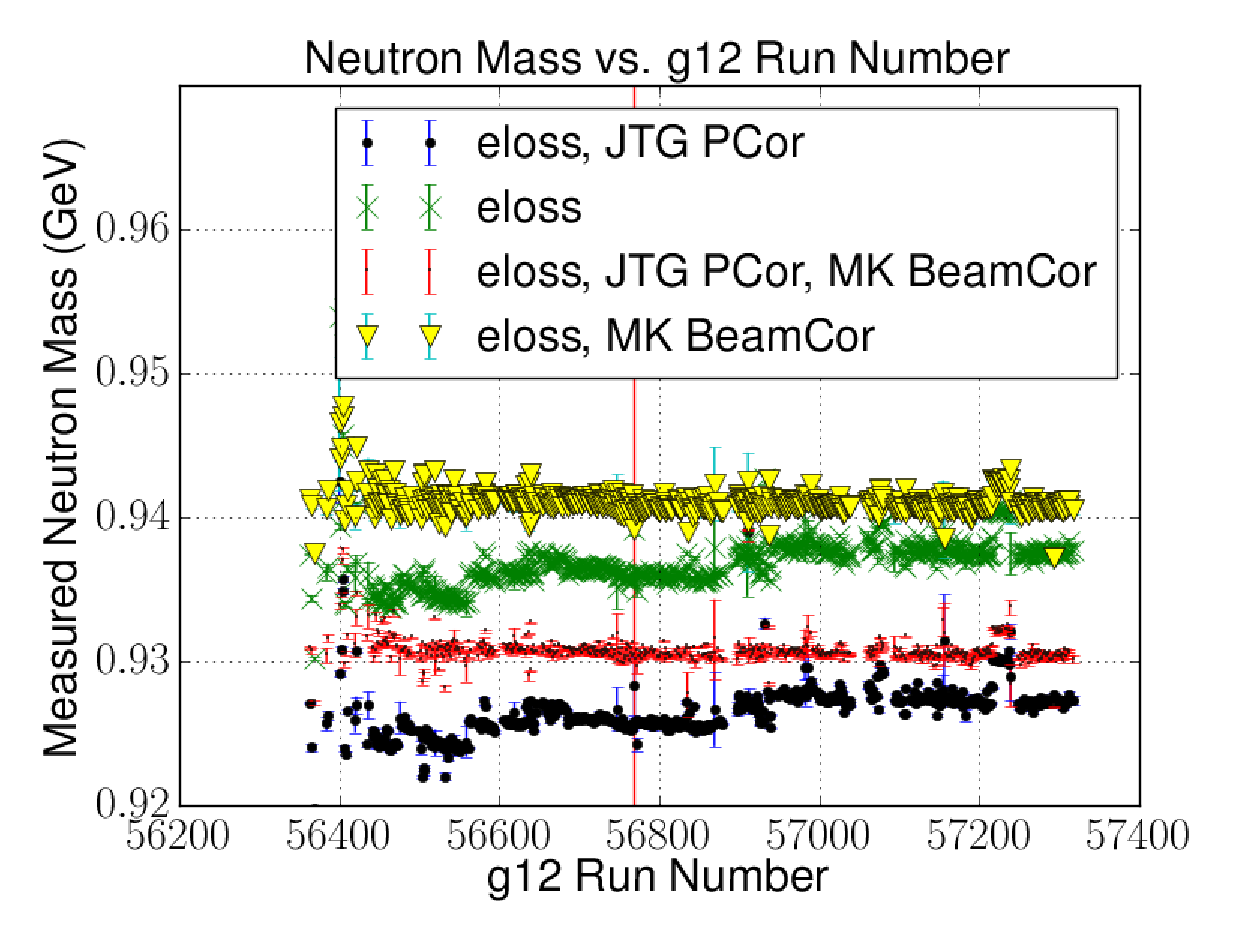
\includegraphics[width=0.6\columnwidth]{figures/corrections/C3pi_allcorr_neutron_rxr.eps}
\caption[Run by run Mass Balance Before and After Corrections]{\label{fig:mbal_pcor}Neutron mass balance of exclusive n \π[+] \π[+] \π[-] events as a function of run number for before corrections, momentum only, beam only, and after both beam and momentum corrections.}
\end{center}\end{figure}


\FloatBarrier


\subsection{\label{sec:data.lepton}General Features of Lepton Data in \desg{g12}}

To identify electrons and positrons properly in \abbr{CLAS}, quantities obtained from the \abbr{CC} and \abbr{EC} are used to reject charged pions. The \abbr{CC} collects the number of photo-electrons caused by Cerenkov radiation and the \abbr{EC} records the energy deposition of electrons/positrons as well as photons. A previous \abbr{CLAS} experiment \desg{g7} analyzed the properties of medium modifications from the decay of vector mesons through the lepton decay channel. This experiment derived a set of cits for identifying electron/positrons pairs in \abbr{CLAS} by employing specific cuts to the number of photo-electrons (\abbr{NPE}) detected in the \abbr{CC}, a match in azimuthal angle $\phi$ from a charged track in the \abbr{DC} to the $\phi$ of the \abbr{CC}, as well as comparing the momentum of the charged track to the energy deposited in the \abbr{EC}. These cuts can be found in Table~\ref{tab:ISLEP_cuts}.
\begin{table}[htpb]
\begin{minipage}{\textwidth}
\begin{center}
\begin{singlespacing}

\caption[Electron/Positron PID Cuts]{\label{tab:ISLEP_cuts}Cuts applied to the \emph{CC} and \emph{EC} to perform electron/positron \emph{PID}. Table source:~\cite{clas.thesis.kunkel} \vspace{0.75mm}}

\begin{tabular}{c|c|c}

\hline
Subsystem & Quantity & Cut \\
\hline
\multirow{2}{*}{\emph{CC}}  & \# of photo-electrons (\emph{NPE})  & \emph{NPE} $>$ 2.5 \\
 &  \emph{DC} $\phi$ \& \emph{CC} $\phi$  & \emph{DC} $\phi$ = \emph{CC} $\phi$ \\
\hline
\multirow{2}{*}{\emph{EC}}  & q$^{\pm}$ momentum threshold (p$\mathrm{_{thres}}$) & \multirow{2}{*}{p$\mathrm{_{thres}^{high}} < \ $E$\mathrm{_{calo}} <$ p$\mathrm{_{thres}^{low}}$ } \\
&  \& \emph{EC} deposited energy (E$\mathrm{_{calo}}$) & \\
\hline \hline
\end{tabular}
\end{singlespacing}
\end{center}
\end{minipage}
\end{table}

To validate the \desg{g7} electron/positron \abbr{PID} scheme for \desg{g12}, a comparison of  the \abbr{CC} and \abbr{EC} quantities was performed for all charged tracks \abbr{CC}/\abbr{EC} hit signatures and while selecting events from π$^0$ decay. To separate the π$^0$ events from the π$^+$π$^-$ events, all charged pions were assigned the mass of electrons and cuts were placed on the missing energy of \mbox{γ p$\rightarrow$p e$^+$ e$^-$} as well as a cut on the missing mass squared of \mbox{γ p$\rightarrow$ p}, values found in Table~\ref{tab:lep_cuts}. A graphical depiction of the cuts applied to separate π$^0$ events from the π$^+$π$^-$ events is seen in Fig.~\ref{fig:islep.cuts}.
\begin{table}[h!]
\begin{minipage}{\textwidth}
\begin{center}
\begin{singlespacing}

\caption[Cuts To Separate $\pi^0$ from $\pi^{+}\pi^{-}$ for \emph{PID} Validation]{\label{tab:lep_cuts}Cuts applied to separate $\pi^0$ events from $\pi^{+}\pi^{-}$ events. Table source:~\cite{clas.thesis.kunkel} \vspace{0.75mm}}

\begin{tabular}{c|c|c}

\hline
Cut Topology & Topology Quantity & Value  \\
\hline
$\gamma p \rightarrow p e^+ e^-$ & Missing Energy ($\mathrm{M_E}$) & $>0.075$~GeV \\
\hline
\multirow{2}{*}{$\gamma p \rightarrow p $}  & \multirow{2}{*}{Missing mass squared ($\mathrm{M_x^2}$)} & $<$ 0.0779~GeV$^2$ for $\pi^0$ events \\
&  & $>$ 0.0779~GeV$^2$ for $\pi^{+}\pi^{-}$ events\\
\hline \hline
\end{tabular}

\end{singlespacing}
\end{center}
\end{minipage}
\end{table}

The values of the threshold momentum are calculated from empirical studies and are based upon calculations using the momentum obtained from the \abbr{DC}$p$ under the following criteria;
\begin{align}
\mathrm{p_{thres}^{low}} = \alpha p *(p+EC_{P\_LO})/p \nonumber \\
\mathrm{p_{thres}^{high}} = \alpha p *(p+EC_{P\_HIGH})/p \nonumber
\end{align}
where $EC_{P\_LO} = -0.3$, $EC_{P\_HIGH} = 0.5$ and
\begin{align}
\alpha p =
\begin{cases}
.23*p + .071p^2 - .032p^3, & p<1.0 \text{~GeV} \\
0.272p, & p>1.0 \text{~GeV} \\
\end{cases}\nonumber
\end{align}


\begin{figure}\begin{center}
\includegraphics[width=0.4\textwidth]{figures/lepton/Lepfeature_cuts.eps}
\caption[Cuts Applied to Isolate π$^0$ and π$^+$ π$^-$ for \abbr{PID} Validation]{\label{fig:islep.cuts}Plot of missing mass squared of off proton (horizontal) vs. missing energy of proton e$^+$e$^-$ (vertical). The red dashed vertical line depicts the π$^+$π$^-$ threshold mass cut while the horizontal red dashed line represents the missing energy cut-off used to sepertate π$^+$π$^-$ from π$^0$.  Image source:~\cite{clas.thesis.kunkel}}
\end{center}\end{figure}

\begin{v2}
There are more and more restrictive cuts one can always do to try to clean up a lepton signal, but the general \abbr{CC}, \abbr{TOF}, and \abbr{EC}$_\mathrm{total}$ are the most robust. After that you can make further cuts on \abbr{EC}$_\mathrm{inner}$ and/or \abbr{EC}$_\mathrm{outer}$ at the users discretion. The g7 lepton cuts were the standard isLepton(), plus a $>45$~MeC \abbr{EC}$_\mathrm{inner}$ cut, see Ref.~\ref{clas.nasseripour}.
\end{v2}

\subsubsection{\label{sec:data.lepton.cc}\abbr{CC} Comparison}

The \abbr{NPE} measured by the \abbr{CC} for all positron/electron (e$^+$/e$^-$) candidates can be seen in Fig~\ref{fig:islep.CC}. The sharp decline prior to 2.5 \abbr{NPE} is due to photo-electrons created by electron/positrons, pions traveling through the \abbr{CC} or pions producing delta-electrons which pass through the \abbr{CC}. Delta-electrons are created as an effect of the ionization of gases that could be present when the pion travels through the \abbr{DC}. These types of electrons are typically lower in momentum than the electrons obtained from particle decays in \abbr{CLAS} and thus should emit less \abbr{NPE} per unit length.

Through mass conservation the particles for the π$^0$ events must be e$^+$/e$^-$ pairs. In comparison to fig.~\ref{fig:islep.CC}, fig.~\ref{fig:islep.CC1} plots the \abbr{NPE} measured by the \abbr{CC} for all e$^+$/e$^-$ pairs for π$^0$ events selected as shown in fig.~\ref{fig:islep.cuts}. It can be seen that the sharp decline prior to \abbr{NPE} = 2.5 is reduced leaving mostly electrons or positrons signatures in the \abbr{CC} concluding that the \desg{g7} \abbr{CC} \abbr{NPE} cut is valid for identifying e$^+$/e$^-$ pairs while rejecting π$^+$/π$^-$ pairs.

\begin{v2}Using the current cuts of \abbr{NPE} and hit angle, the suppression of di-leptons was sufficient without including additional cuts on the \abbr{CC} such as a timing comparison to the \abbr{TOF}. This method of lepton \abbr{PID}, involving di-leptons, was established during the \textit{g7} run period. Further \textit{g12} analyses that involve single lepton \abbr{PID} could include this as a cut.\end{v2}

%
\begin{figure}\begin{center}
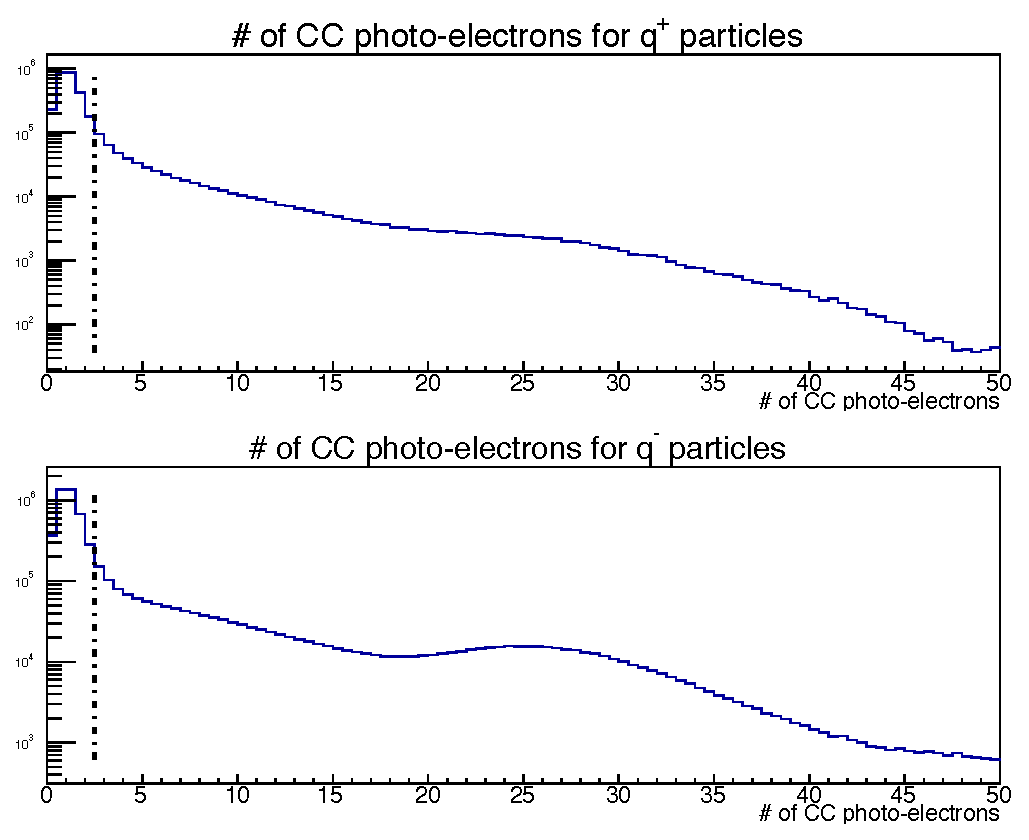
\includegraphics[width=0.4\textwidth]{figures/lepton/CC_nPE.eps}
\caption[Number of Photo-electrons Measured by \abbr{CC} for All e$^-$ and e$^+$ Candidates]{\label{fig:islep.CC}Plot of \abbr{NPE} measured by \abbr{CLAS} \abbr{CC} subsystem for positron/electron candidates top/bottom respectively. The dashed dotted vertical line depicts the cut applied if using the \desg{g7} lepton \abbr{PID} scheme. Image source:~\cite{clas.thesis.kunkel}}
\end{center}\end{figure}

\begin{figure}\begin{center}
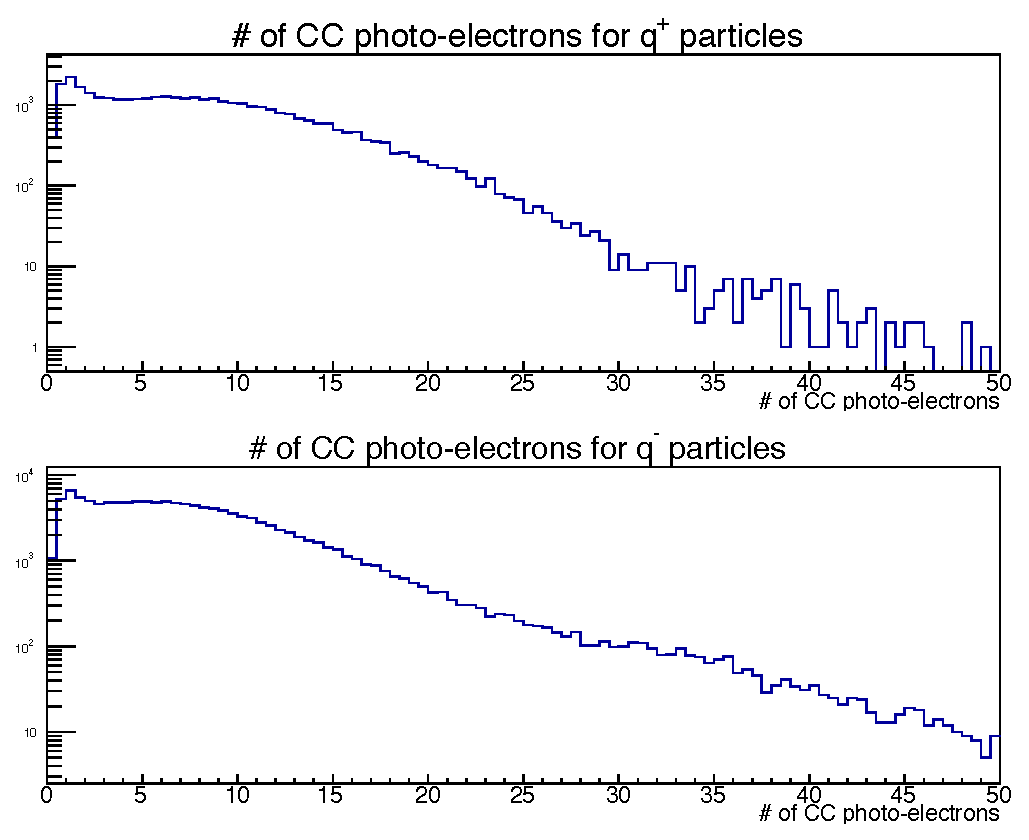
\includegraphics[width=0.4\textwidth]{figures/lepton/CC_NPEcut.eps}
\caption[Number of Photo-electrons Measured by \abbr{CC} for π$^0$ Events]{\label{fig:islep.CC1}Plot of \abbr{NPE} measured by \abbr{CLAS} \abbr{CC} subsystem when selecting π$^0$ events seen in Fig~\ref{fig:islep.cuts}, positron/electron candidates top/bottom respectively. Image source:~\cite{clas.thesis.kunkel}}
\end{center}\end{figure}

\FloatBarrier






\subsubsection{\label{sec:data.lepton.ec}\abbr{EC} Comparison}

Similarly to the \abbr{CC} comparison, figures~\ref{fig:islep.pimEClow},~\ref{fig:islep.pimEChigh},~\ref{fig:islep.pipEClow},~\ref{fig:islep.pipEChigh} depict the  p$\mathrm{_{thres}^{low}}$ and  p$\mathrm{_{thres}^{low}}$ cuts listed in  Table~\ref{tab:ISLEP_cuts} for the q$^-$ and q$^+$ tracks respectively. After π$^0$ event selection, seen in figures~\ref{fig:islep.pimEC},~\ref{fig:islep.pimECcut} ,~\ref{fig:islep.pipEC} ,~\ref{fig:islep.pipECcut}, the bulk of e$^+$/e$^-$ events reside within the region of the cut acceptance therefore it is evident that the \desg{g7} \abbr{EC} cuts are valid for identifying e$^+$/e$^-$ pairs. The following four plots are for electron($e^-$) \abbr{PID} validation of the \desg{g7} \abbr{EC} cuts described in Table~\ref{tab:ISLEP_cuts}.
%
\begin{figure}\begin{center}
\includegraphics[width=0.4\textwidth]{figures/lepton/Pim_EClow.eps}
\caption[\abbr{EC} Deposited Energy Comparison to Lower Threshold Track Momentum for q$^-$ Tracks]{\label{fig:islep.pimEClow}Plot of energy deposited measured by \abbr{EC} vs. track momentum p$\mathrm{_{thres}^{low}}$ for negative charged tracks. The red region depicts the cut that would reject events in the \desg{g7} lepton \abbr{EC} \abbr{PID} scheme. Image source:~\cite{clas.thesis.kunkel}}
\end{center}\end{figure}

\begin{figure}\begin{center}
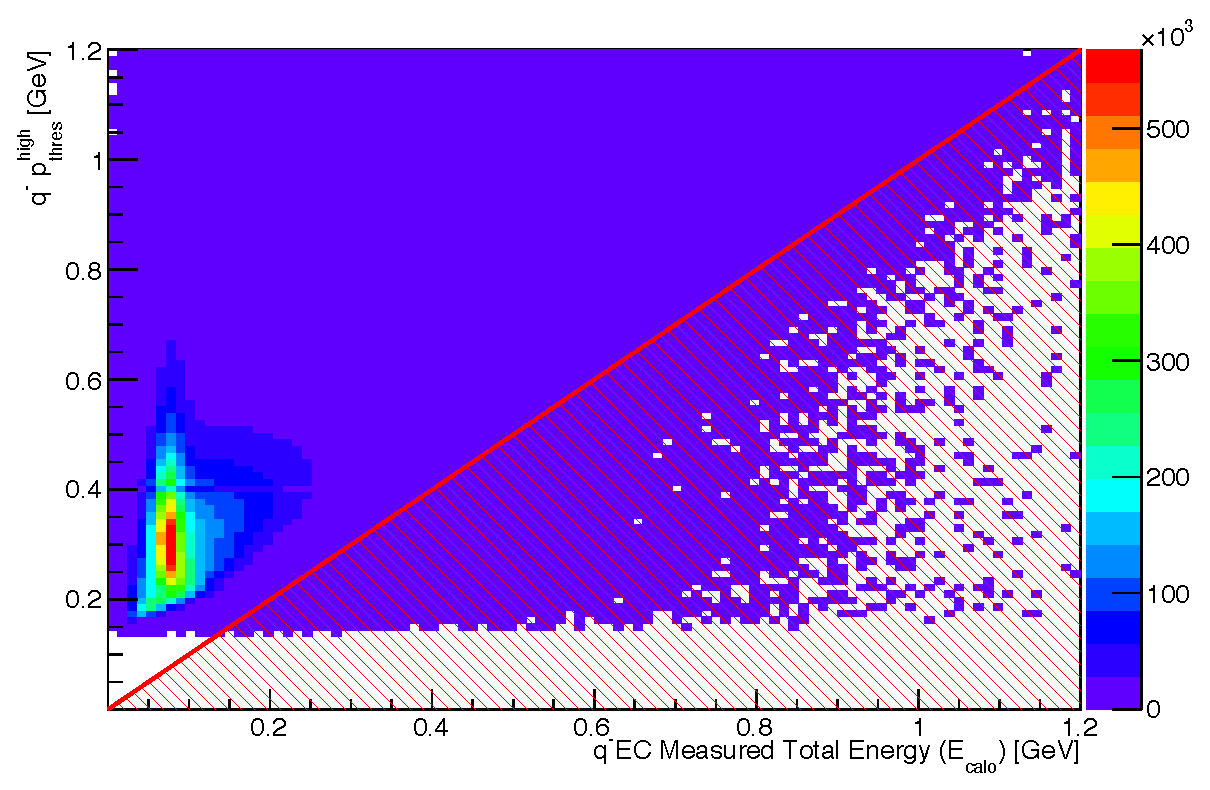
\includegraphics[width=0.4\textwidth]{figures/lepton/Pim_EChigh.eps}
\caption[\abbr{EC} Deposited Energy Comparison to Upper Threshold Track Momentum for q$^-$ Tracks]{\label{fig:islep.pimEChigh}Plot of energy deposited measured by \abbr{EC} vs. track momentum p$\mathrm{_{thres}^{high}}$ for negative charged tracks. The red region depicts the cut that would reject events in the \desg{g7} lepton \abbr{EC} \abbr{PID} scheme. Image source:~\cite{clas.thesis.kunkel}}
\end{center}\end{figure}


\begin{figure}\begin{center}
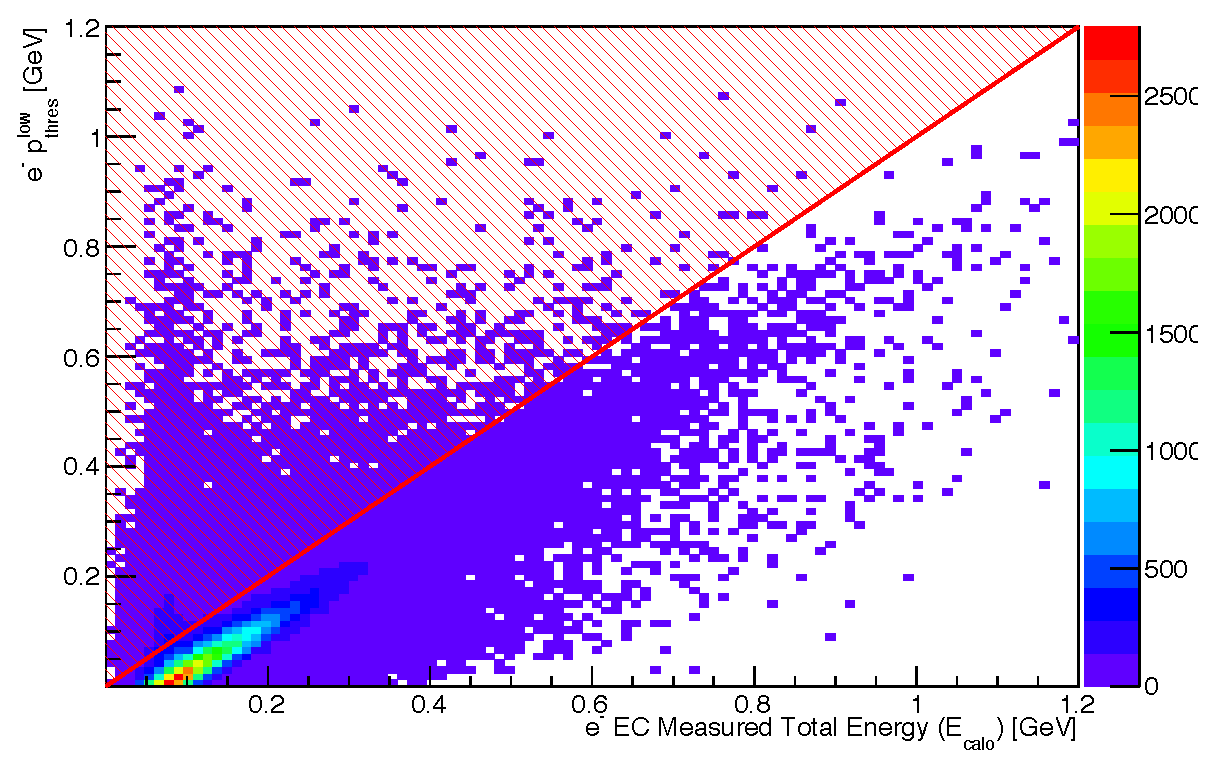
\includegraphics[width=0.4\textwidth]{figures/lepton/Pim_EClowcut.eps}
\caption[\abbr{EC} Deposited Energy Comparison to Track Momentum for e$^-$ Candidates]{\label{fig:islep.pimEC}Plot of energy deposited measured by \abbr{EC} vs. track momentum p$\mathrm{_{thres}^{low}}$ for electrons from π$^0$ events without the \desg{g7} lepton \abbr{EC} \abbr{PID} scheme applied. The red region depicts the cut that would reject events in the \desg{g7} lepton \abbr{EC} \abbr{PID} scheme. Image source:~\cite{clas.thesis.kunkel}}
\end{center}\end{figure}

\begin{figure}\begin{center}
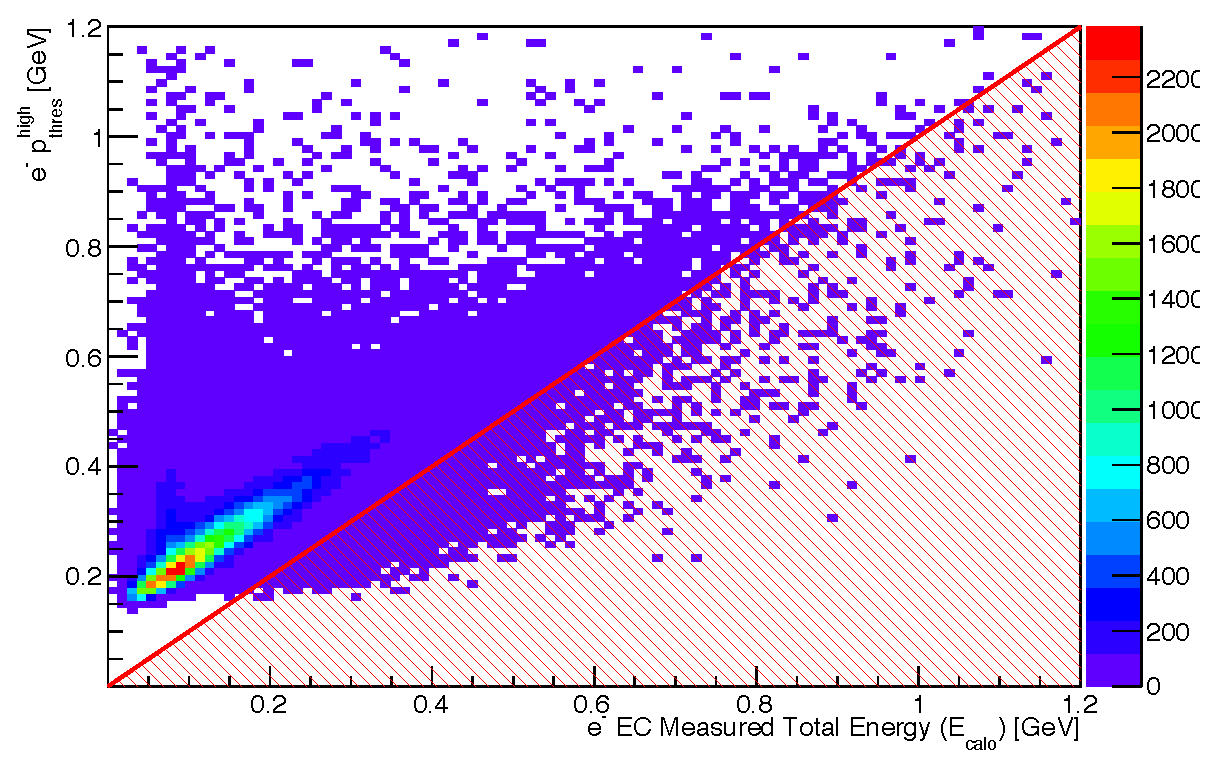
\includegraphics[width=0.4\textwidth]{figures/lepton/Pim_EChighcut.eps}
\caption[\abbr{EC} Deposited Energy Comparison to Track Momentum for e$^-$ from π$^0$ Events]{\label{fig:islep.pimECcut}Plot of energy deposited measured by \abbr{EC} vs. track momentum p$\mathrm{_{thres}^{high}}$ for electrons from π$^0$ events without the \desg{g7} lepton \abbr{EC} \abbr{PID} scheme applied. The red region depicts the cut that would reject events in the \desg{g7} lepton \abbr{EC} \abbr{PID} scheme. Image source:~\cite{clas.thesis.kunkel}}
\end{center}\end{figure}

Figures~\ref{fig:islep.pipEClow}--\ref{fig:islep.pipECcut} are for positron (e$^+$) \abbr{PID} validation of the \desg{g7} \abbr{EC} cuts described in Table~\ref{tab:ISLEP_cuts}.

\begin{figure}\begin{center}
\includegraphics[width=0.45\columnwidth]{figures/lepton/Pip_EClow.eps}
\caption[\abbr{EC} Deposited Energy Comparison to Lower Threshold Track Momentum for q$^+$ Tracks]{\label{fig:islep.pipEClow}Plot of energy deposited measured by \abbr{EC} vs. track momentum p$\mathrm{_{thres}^{low}}$ for positive charged tracks. The red region depicts the cut that would reject events in the \desg{g7} lepton \abbr{EC} \abbr{PID} scheme. Image source:~\cite{clas.thesis.kunkel}}
\end{center}\end{figure}

\begin{figure}\begin{center}
\includegraphics[width=0.45\columnwidth]{figures/lepton/Pip_EChigh.eps}
\caption[\abbr{EC} Deposited Energy Comparison to Upper Threshold Track Momentum for q$^+$ Tracks]{\label{fig:islep.pipEChigh}Plot of energy deposited measured by \abbr{EC} vs. track momentum p$\mathrm{_{thres}^{high}}$ for positive charged tracks. The red region depicts the cut that would reject events in the \desg{g7} lepton \abbr{EC} \abbr{PID} scheme. Image source:~\cite{clas.thesis.kunkel}}
\end{center}\end{figure}

\begin{figure}\begin{center}
\includegraphics[width=0.45\columnwidth]{figures/lepton/Pip_EClowcut.eps}
\caption[\abbr{EC} Deposited Energy Comparison to Track Momentum for e$^+$ Candidates]{\label{fig:islep.pipEC}Plot of energy deposited measured by \abbr{EC} vs. track momentum p$\mathrm{_{thres}^{low}}$ for positrons from π$^0$ events without the \desg{g7} lepton \abbr{EC} \abbr{PID} scheme applied. The red region depicts the cut that would reject events in the \desg{g7} lepton \abbr{EC} \abbr{PID} scheme. Image source:~\cite{clas.thesis.kunkel}}
\end{center}\end{figure}

\begin{figure}\begin{center}
\includegraphics[width=0.45\columnwidth]{figures/lepton/Pip_EChighcut.eps}
\caption[\abbr{EC} Deposited Energy Comparison to Track Momentum for e$^+$ from π$^0$ Events]{\label{fig:islep.pipECcut}Plot of energy deposited measured by \abbr{EC} vs. track momentum p$\mathrm{_{thres}^{high}}$ for positrons from π$^0$ events without the \desg{g7} lepton \abbr{EC} \abbr{PID} scheme applied. The red region depicts the cut that would reject events in the \desg{g7} lepton \abbr{EC} \abbr{PID} scheme. Image source:~\cite{clas.thesis.kunkel}}
\end{center}\end{figure}



\FloatBarrier


\section{Flux Determination}

The photon flux is based on the flux procedure outline in Ref. \cite{clas.flux}. The script to generate the photon flux for g12 is here:
\begin{align}
    \texttt{/home/clasg12/local/scripts/g12-gflux} \nonumber
\end{align} and there is also a script (/home/clasg12/local/scripts/g12-gflux-all) that doesn't rebin the energies and outputs two columns: energy and flux for each logical paddle in the tagger.

The help output from the script:
\begin{verbatim}
> /home/clasg12/local/scripts/g12-gflux -h
usage: g12-gflux emin emax ebinwidth runlist.txt (good|all)
    (good|all) specifies either all scalar intervals
    or only "good" scalar intervals.
example:
     g12-gflux 1.5 5.5 0.2 runlist.txt good
where runlist.txt is an ascii file of one column: run
56363
56365
...
\end{verbatim}

To use the script, you will need to create a file that consists of the run numbers you used in your analysis. Using this filename when you call g12-gflux, will give you the total flux as a function of beam energy in the range and binning requested. The command:
\begin{verbatim}
/home/clasg12/local/scripts/g12-gflux 1.5 5.5 0.2 filelist.txt good
\end{verbatim}

will return to stdout the flux in the energy bins using three columns: emin, emax, flux. Something like this:
\begin{verbatim}
1.5 1.7 7.75466725993e+12
1.7 1.9 7.23861294572e+12
1.9 2.1 6.85242336788e+12
... [snip] ...
4.9 5.1 2.69244768955e+12
5.1 5.3 2.49808049501e+12
5.3 5.5 1.99322166816e+12
\end{verbatim}

The option good or all can be used to specify if you only want to consider good regions, throwing out beam trips, or if you want all events from good scalar intervals as well as the beam trip regions.

An alternative script which doesn't rebin the data but returns the flux for each logical energy paddle can be run like this:
\begin{verbatim}
/home/clasg12/local/scripts/g12-gflux-all filelist.txt good
\end{verbatim}
The script has been extensively tested on the 64-bit machines. The precision of all variables are adequate to provide at least 4 significant figures for the final flux numbers. The two scripts both poll the flux information from the output files of the program \prog{gflux} which was run with the options:
\begin{verbatim}
gflux -c -b -B -ooutput.hbook -ttripfile.txt -F100000 -f0 -l1000 <infiles>
\end{verbatim}
where \verb+<infiles>+ included all files, in order, for a specific run. The output files are kept on the \verb+/work+ directory on the CUE machines at JLab here:
\begin{verbatim}
/work/clas/clasg12/flux
\end{verbatim}
and the associated trip files (see discussion below in Sec.~\ref{sec:flux.trips}) can be found here:
\begin{verbatim}
/work/clas/clasg12/clasg12/tripfiles
\end{verbatim}
For reference, the output of \verb+gflux -h+ is here:
\begin{verbatim}
Usage: gflux [-Options] file1 [file2] etc...

  Options:
    -B          Bloated mode(All histograms) equivalent to -P -T -e
    -F[#]       Run gated clock frequency in KHz, default 10 KHz
    -M[#]       Process only # number of events
    -N[#]       Normalize to this run, instead of using map
    -P          Rebuild PID with particle histograms
    -R          Do NOT rebuild TAGR bank, by default it does
    -T          Raw tagger histograms from TAGE, TAGT, and TAGI

    -E          apply tagger energy correction (default: no correction)

    -b          Batch mode(no printout on screen)
    -c          Clock based DAQ livetime, default event based
    -e          Make exclusive reaction histograms
    -f          File number, necessary if you want to keep txt files
    -l[#]       Scaler intervals in timeline histograms, default 50
    -n          Process a normalization run
    -o<outfile> Output hbook file name
    -p          Particle histograms without rebuilding PID
    -p          Particle histograms without rebuilding PID
    -s          Start counter histograms from ST1 and STR
    -t<file>    Trip file
    -y<file>    Synch event mode (skip events)
\end{verbatim}

The major caveat to using this script, which relies on \prog{gflux}, is that you must included \emph{whole runs} in your analysis for this to be accurate. This is because the \prog{gflux} program was not designed to work with partial runs. So, you must verify that you have processed every file in the runs which were analyzed -- one can use the \prog{g12runs} program to aid in this.

\subsection{\label{sec:flux.trips}Beam Trips}

Beam trips were classified as scalar intervals with a lifetime above a threshold of 0.90. Depending on the trigger and run conditions, the peak of the lifetime ranged from 0.85 to 0.80. Additionally, due to the setup of the program in the flux procedure outline, Ref. \cite{clas.flux.note}, the beginning and the end of every file was labeled a bad scalar interval. With such a high number of files per run (100 to 200 files), roughly $12\%$ of good data would be lost. To remedy this, we were able to load and run the flux calculator on a whole run basis and recover most of the events except for the first and last scalar of the run. As a result the flux is valid for whole runs only and a proper run list can be obtained from the g12-flux script.

\FloatBarrier


\subsection{\label{sec:flux.normyields}Normalized Yields for Different Beam Conditions}
The beam current study that took place from runs 56363 to 56519 had beam currents ranging from 5 to 90 nA. These runs used a preliminary 2-prong trigger. This data is from $E_{\gamma}$ > 4.4 GeV. The fit shows a slope to the beam currents with an error larger than the slope.

\begin{figure}[h]
\begin{center}
 \includegraphics[width=0.9\textwidth]{figures/gflux/gflux_bycurrent_omega.eps}
  \caption{Photon flux normalized yields by current for the beam current study runs (Runs < 56519).}
  \label{gfluxbycurrent}
  \end{center}
\end{figure}
\FloatBarrier



\subsection{\label{sec:flux.runbyrun}Run-by-run Stability and Systematic Uncertainty of Flux}
This run by run plot shows the stability of the flux corrections for runs after run 56519. These runs all use the same trigger and have a cut on $E_{\gamma}$ > 4.4 GeV. 

\begin{figure}[h]
\begin{center}
 \includegraphics[width=0.9\textwidth]{figures/gflux/gflux_runstability_omega.eps}
  \caption{Photon flux normalized yields by run for the production runs (Runs > 56519).}
  \label{gfluxbyrun}
  \end{center}
\end{figure}

\FloatBarrier

\section{\label{sec:sim}Simulations}

All the programs in this section can be obtained from the standard \desg{SVN} repository for \desg{CLAS} here:
\begin{center}
    \url{https://jlabsvn.jlab.org/svnroot/clas/trunk}
\end{center}
Under this directory, you may find the following directories which hold the programs in the order which they appear below:
\begin{itemize}
    \item \prog{simulation/generators/genr8}
    \item \prog{io/part2gamp}
    \item \prog{io/bosdump}
    \item \prog{simulation/generators/ppgen}
    \item \prog{simulation/gsim}
    \item \prog{simulation/gpp}
\end{itemize}

\subsection{\label{sec:sim.gen}Generating Events for Digitization}

One may use the program \texttt{genr8} for generating t-channel phase space events. It is driven by an input key file which describes the exclusive reaction. Typical usage to generate 10k events from 4.4 to 5.45~GeV in beam energy using the input file ``\verb+n_pi-pi+pi+.input+'' looks like this:
\begin{verbatim}
genr8 -M10000 -B4.4,5.45 -oevents.gamp < n_pi-pi+pi+.input
\end{verbatim}
See the genr8 documentation for how to write the input file, or you can see this example here:
\begin{align}
    \texttt{http://clasweb.jlab.org/rungroups/g12/wiki/index.php/N\_pimpippip} \nonumber
\end{align}

Gsim requires a bos file with a PART bank containing the MC event. Note PART bank 0 is reserved for MC events whereas PART banks 1 and 2 are used for containing the reconstructed event. The best way to convert GAMP to PART banks is by using gamp2part -- the command, for protons pions and kaons, following the example above is:
\begin{verbatim}
gamp2part -r56855 -oevents.part -T -S-0.321,0.378,-0.254,0.407 \
  -z-110,-70 events.gamp
\end{verbatim}
and for electrons and positrons
\begin{verbatim}
gamp2part -r10 -oevents.part -T -S-0.321,0.378,-0.254,0.407 \
  -z-110,-70 events.gamp
\end{verbatim}
where the option -r10 is specific to RUN 10 in:
\begin{verbatim}
export CLAS_CALDB_RUNINDEX=calib_user.RunIndexg12_mk
\end{verbatim}
This writes a BOS file full of PART, sector 0 banks with the 4-vector information from the gamp file. Also, the -z option smears the target distribution in Z, while the -S smears it in X and Y. The parameters are means and sigmas of a 2D Gaussian which were derived from a fit to the data. An alternative way to convert a gamp file to a BOS PART bank file is using gamp2txt and txt2part. These programs are piped together during run time.
\begin{verbatim}
gamp2txt -E5.714 -z-110,-70 < events.gamp | txt2part -T -oevents.part
\end{verbatim}
The above command takes in gamp events, smears the z vertex in the target range, creates a tagger hit and writes out a bos file with HEAD, PART, and TAGR banks. Here is a bosdump of an event:
\begin{verbatim}
ifarml1> bosdump events.part -M1
Group:  HEAD    Sector: 0       Nhits:  1   Next ind:    0

Version:        0
Run:            1
Event:          1
Type:           -2  (GSIM monte carlo)
ROC:            0
CLASS:          15
Trgbit:         0x1
TIME:           Wed Feb 27 22:16:00 2008


Group:  PART    Sector: 0       Nhits:  3  Next ind:       0
pid:   8
   vert-> x: 0.000  y: 0.000  z: -95.178
   p-> E: 3.194  px: -0.591  py: -0.688  pz: 2.942
   q: 1.000  trkid:   0  qpid: 0.000  qtrk:  0  flags:   0
pid:   9
   vert-> x: 0.000  y: 0.000  z: -95.178
   p-> E: 3.194  px: -0.591  py: -0.688  pz: 2.942
   q: -1.000  trkid:   0  qpid: 0.000  qtrk  0  flags:   0
pid:   8
   vert-> x: 0.000  y: 0.000  z: -95.178
   p-> E: 4.780  px: -0.246  py: -0.140  pz: 4.383
   q: 1.000  trkid:   0  qpid: 0.000  qtrk:   0  flags:   0

Group:  TAGR    Sector: 0       Nhits:  1  Next ind:      0
ERG:5.001 TTAG:0.000  TPHO:0.000 STAT:15 T_id:17  E_id:82
\end{verbatim}

One can use any alternative to \texttt{genr8} as long as the output is either gamp or an appropriate BOS file. For example, there is the phase-space generator \texttt{ppgen}:
\begin{verbatim}
ppgen -M<reaction code> -P<photon energy> -E5.714 -j1 -G -A \
  -t<t-slope> -m50000 > events.gamp
\end{verbatim}
The output can be txt or gamp file depending on user's needs. Follow the previous instructions to convert to part banks as needed.

\subsection{\label{sec:sim.digit}Digitization and Smearing}

The program to track the particles through the simulation and ultimately digitize the information to simulated ``raw'' banks is the geant3-based program: \texttt{gsim}. Running this on the BOS file created above looks like this:
\begin{verbatim}
gsim_bat -ffread ffread.g12 -kine 1 -mcin events.part \
  -bosout events.gsim -trig 2000000
\end{verbatim}
Using the above command, should create a gsim BOS output file. Here is the FFREAD file should be used to run gsim\_bat for \desg{g12} analyses not using electrons/positrons:
\begin{verbatim}
===BEGIN=====FFREAD.G12======================
CUTS   5.e-3 5.e-3 5.e-3 5.e-3 5.e-3
DCCUTS 1.e-4 1.e-4 1.e-4 1.e-4 1.e-4
ECCUTS 1.e-4 1.e-4 1.e-4 1.e-4 1.e-4
SCCUTS 1.e-4 1.e-4 1.e-4 1.e-4 1.e-4

MAGTYPE 2
MAGSCALE 0.500 0.000
PTGIFIELD 0
STTYPE 1
STZOFF -90.0
TGPOS 0. 0. 0.
TARGET 'g11a'
TGMATE 'PROT'
POSBEAM 0.0 0.0

GEOM 'ALL' 'ST'
NOGEOM 'MINI' 'PTG '
BEAM 0 0 5.714
DCAY 1
KINE 1
MULS 1
AUTO 1

RUNG 56855
TIME 1000000 1000000 1000000
TRIG 1000000
STOP
===END=====FFREAD.G12=======================
\end{verbatim}
and for electrons/positrons the FFREAD file should read
\begin{verbatim}
=============FFREAD.G12======================
CUTS   5.e-3 5.e-3 5.e-3 5.e-3 5.e-3
CCCUTS 1.e-3 1.e-3 1.e-3 1.e-3 1.e-3
DCCUTS 1.e-4 1.e-4 1.e-4 1.e-4 1.e-4
ECCUTS 1.e-4 1.e-4 1.e-4 1.e-4 1.e-4
SCCUTS 1.e-4 1.e-4 1.e-4 1.e-4 1.e-4

UPSTPOS 0. 0. 0.
MAGTYPE 2
MAGSCALE 0.500 0.000
PTGIFIELD 0
STTYPE 1
STZOFF -90.0
TGPOS 0. 0. 0.
TARGET 'g11a'
TGMATE 'PROT'
POSBEAM 0.0 0.0
GEOM 'ALL' 'ST'
NOGEOM 'MINI' 'PTG'
BEAM00 5.714
DCAY 1
PAIR 1
HADR 1
MULS 1
KINE 1
AUTO 1
RUNG 10
TRIG 200000
STOP
============================================
\end{verbatim}
The tracking and digitization done by \texttt{gsim} is ideal and there is no smearing done. To get the simulated data to mimic the detector resolution the ``gsim post-processor'' (\texttt{gpp}) is used. For \desg{g12}, and following the above example, one should use this command for protons, pions and kaons:
\begin{verbatim}
gpp -Y -s -S -a2.73 -b1.7 -c1.93.-f1 -R56855 -P0x7f -oevents.gpp events.gsim
\end{verbatim}
and for electrons and positrons
\begin{verbatim}
gpp -Y -s -S -a2.73 -b1.7 -c1.93.-f1 -R10 -P0x7f -oevents.gpp events.gsim
\end{verbatim}
The values passed to the gpp command line options, -a, -b, -c, helps match the tracking resolution of the simulated data to that of the real events in the regions 1,2 and 3 of the CLAS Drift Chambers. They accomplish this by smearing the DOCA values and hence gpp is able to match the DC residuals for the simulated CLAS tracks to that of the real CLAS tracks on a region-by-region basis. The gpp option -f smears the Time-of-Flight tdc values and during analysis the default gpp smearing for TOF was found to be adequate. The smearing should be run with a good g12 run number; run 56855 has all the necessary constants in the database to get the tagger timing smearing done correctly. Also, interested parties can add accidentals to the TAGR bank by using the -A option like so:
\begin{verbatim}
gpp -Y -s -S -a2.73 -b1.7 -c1.93 -f1 -R56855 -P0x7f -oevents.gpp \
  -A/path/to/output/from/filter_tagr events.gsim
\end{verbatim}
The program \texttt{filter\_tagr} scans through real data files and outputs a bos file containing only the TAGR banks. These files are then supplied to gpp with the -A option, and gpp puts the contents of these banks as accidentals in the MC TAGR bank. Output from \texttt{filter\_tagr} for run 56855 can be found at:
\begin{align}
    \texttt{/home/clasg12/local/etc/clas6/gpp\_tagger\_profile.bos} \nonumber
\end{align}


As stated earlier, the goal of using GPP is to simulate the experimental conditions as close as possible. So we smear the values of the DOCA for the simulated tracks with a single Gaussian whose width is equal to the events weighted sum of the widths of the two Gaussians fitted to the data from the run 56855. This makes the residual for a superlayer in the simulated data approximately equal to the weighted residual from the real data. The default available options for GPP specifies only three parameters `-a, -b, -c' for DC DOCA smearing, where each parameter is responsible for the smearing of two superlayers (in one Region) of all six sectors. Hence, we choose a set of parameters based on the following fits as seen in Figs.~\ref{fig:SLRes} and \ref{fig:SLRes_default}, which gives us the best match on average between the different superlayers in the six sectors (see Fig.~\ref{fig:DC_SL_Match}).

\begin{figure}[htpb]\begin{center}
\includegraphics[width=0.8\columnwidth]{figures/calib/dc/Sector_1_compare.eps}
\caption[DC superlayers Resolution Matching]{\label{fig:SLRes}Plots and Fits used to match the residuals (resolution) for Drift Chamber superlayers in CLAS Sector 1, between the Data and the Simulation. Data is an empirical fit to a convolution of two gaussians. The simulated distribution is a single gaussian with its simulated width approximately equal to the weighed sum of the widths of the two gaussians fitted to the data. This simulation uses the best estimated smearing parameters to match the DC residuals, between the Data and the Simulation.}
\end{center}\end{figure}

\begin{figure}[htpb]\begin{center}
\includegraphics[width=\columnwidth]{figures/calib/dc/Sector_1_compare_default.eps}
\caption[DC superlayers Resolution Matching]{\label{fig:SLRes_default}Plots and Fits used to compare the residuals (resolution) for Drift Chamber superlayers in CLAS Sector 1, between the Data and the Simulation using the default GPP smearing.}
\end{center}\end{figure}

\begin{figure}[htpb]\begin{center}
\begin{subfigure}{0.47\columnwidth}
    \includegraphics[width=\columnwidth]{figures/calib/dc/DC_Sigma_SL.eps}
    \label{fig:DC_SL_best}
\end{subfigure}
\begin{subfigure}{0.47\columnwidth}
    \includegraphics[width=\columnwidth]{figures/calib/dc/DC_Sigma_SL_default.eps}
    \label{fig:DC_SL_default}
\end{subfigure}
\caption[DC superlayers Resolution Matching]{\label{fig:DC_SL_Match}Comparison of the DC residuals on a superlayer basis for all the CLAS sectors for real as well as simulated events. The left plots use the best estimated smearing parameters for the DC DOCA to match the real and simulated data shown in Figure~\ref{fig:SLRes}., whereas the right plots use the default GPP smearing shown in Figure~\ref{fig:SLRes_default}.}
\end{center}\end{figure}

The smearing parameter `-f' for the Time of Flight timing resolution is one of the GPP parameters that is usually used to match the quality of data and simulation. Using the reference run 56855, we observe that the default GPP smearing is adequate (see Figure \ref{fig:TOF_Res}).

\begin{figure}[htpb]\begin{center}
\includegraphics[width=\columnwidth]{figures/calib/dc/TOF_Compare.eps}
\caption[TOF Resolution Matching]{\label{fig:TOF_Res}Plots and Fits used to match the TOF timing resolution. The default smearing of GPP was found to be adequate in this case.}
\end{center}\end{figure}

These smearing parameters affect the reconstruction efficiency for the tracks in CLAS during simulations. A rudimentary analysis quantifying the effect is presented in Table~\ref{tab:recon.eff}. As expected, as the Drift chamber response becomes more noisy due to smearing of DOCA (higher DC residuals), the reconstruction and tracking efficiency in CLAS goes down.

\begin{table}
\begin{center}
\begin{minipage}{\textwidth}
\caption{\label{tab:recon.eff} Measure of Track Reconstruction Efficiency for sets of \texttt{gpp} parameters}
\begin{center}
\begin{tabular}{ccccccc}
\hline \hline
Events & Events & Reconstruction & \multicolumn{4}{c}{\prog{gpp} Smearing Factors} \\
Generated  &  Accepted  & Acceptance & -a & -b & -c & -f \\
\hline
90000 & 1217 & 1.352\% & 1     & 1   & 1    & 1 \\
90000 & 1161 & 1.29\%  & 2.73  & 1.7 & 1.93 & 1 \\
90000 & 1053 & 1.17\%  & 2.73  & 1.7 & 1.93 & 2 \\
\hline \hline
\end{tabular}
\end{center}
\end{minipage}
\end{center}
\end{table}

\subsection{\label{sec:sim.recon}Reconstruction of Simulated Data}

The reconstruction of simulated data requires a slightly different tracking function and is taken care of by adding the option \verb+-X0+ to the reconstruction program. For protons, pions and kaons:
\begin{verbatim}
a1c -T4 -ct1930 -cm0 -cp0 -X0 -d1 -F -P0x1bff -z0,0,-90 \
    -Aprlink_tg-90pm30.bos -oevents.a1c events.gpp
\end{verbatim}
and for electrons and positrons:
\begin{verbatim}
a1c -R10 -T4 -ct1930 -cm0 -cp0 -X0 -d1 -F -P0x1bff -z0,0,-90 \
    -Aprlink_tg-90pm30.bos -oevents.a1c events.gpp
\end{verbatim}
The help output of \prog{a1c} says this about the \verb+-X#+ option:
\begin{verbatim}
    [-X#]    use a different x vs. t function in tracking (def = 2, MC = 0)
\end{verbatim}

\FloatBarrier

\subsection{\label{sec:fiducial}Fiducial Region Selection}

We derived \emph{Geometric fiducial cuts} for the g12 data, which are cuts based on the exclusion of events laying outside regions where acceptance is well behaved and reliably reproduced in simulation. Such regions for all g12 data are expressed as an upper and lower limit of the difference in azimuthal angle between the center of a given sector, and a particle track.  Because of the hyperbolic geometry of CLAS and the presence of the toroidal magnetic field, the fiducial boundaries on the angle $\phi$ are functions of momentum ($p$), charge, and polar angle ($\theta$) of each track. The boundaries were evaluated separately in each sector, nominally defined as the $\phi$ values in which occupancy drops below 50\% of that in the respective sector's flat region. The flat regions were defined as $-10^{\circ} < \phi < 10^{\circ}$. The nominal upper and lower $\phi$ limits depend strongly on particle charge, $p$ and $\theta$, hence the need for functional characterization and extrapolation.

In order to determine the fiducial limits for charged hadrons, a sample of exclusive \mbox{γ π$\to$p \π[+] \π[-]} events were sliced into $5\times15\times6$ bins in $p$, $\theta$, and sector respectively. The $\phi$ distributions for \π[+] and \π[-] were plotted separately in each bin. The upper and lower $\phi$ limits of these \emph{first-generation} plots were found according to the nominal fiducial definition of 50\% occupancy as illustrated in Fig.~\ref{gen12}. The results from the first-generation fits were represented in \emph{second-generation} plots of $\phi_{min}$ and $\phi_{max}$ vs $\theta$ as also shown in Fig.~\ref{gen12}.  The data in the second-generation plots were fit with hyperbolas, chosen since they replicate the projection of the detector.  Second-generation fitting parameters were then plotted vs $p$ in \emph{third-generation} plots. These third generation plots were fit to power functions as shown in Fig.~\ref{gen3}. Results of the third-generation fits define the sought after functional form $\phi_{min}(\theta,p)$ and $\phi_{max}(\theta,p)$ for each sector. The sector integrated results for positive and negative hadron tracks compose the nominal fiducial region. \emph{Tight cuts} and \emph{loose cuts} were defined as a contraction and expansion respectively, by $4^\circ$ from the nominal fiducial cuts. Figs.~\ref{figures/fiducial/fid2}-\ref{figures/fiducial/fid5} show the effects of the cuts.

\begin{figure}
\includegraphics[width=0.48\linewidth]{figures/fiducial/gen1}
\includegraphics[width=0.48\linewidth]{figures/fiducial/gen2}
\caption{Left: shows the \π[+] $\phi$ distribution for sector-three in one $p$ and $\theta$ bin along with the upper and lower limits of the fiducial region represented by the green vertical line. Right: a second-generation plot, fit to a hyperbola.}
\label{gen12}
\end{figure}

\begin{figure}
\includegraphics[width=0.48\linewidth]{figures/fiducial/3a}
\includegraphics[width=0.48\linewidth]{figures/fiducial/3b}
\caption{Third-generation plots of the fitting parameters from second-generation fits for sector three. The data are fit to power functions.}
\label{gen3}
\end{figure}




\newcommand{\onefig}[3]{
\begin{figure}
    \centering
    \includegraphics[width=#1\textwidth]{#2}
    \caption{#3}
    \label{#2}
    \end{figure}
}


\onefig{0.6}{figures/fiducial/fid2}{The angular distribution of the proton from exclusive \mbox{p \π[+] \π[-]} events is shown.  In the top, $\phi$ vs $\theta$ is plotted, the bottom plots conveys similar information mapped to mimic the geometry of CLAS. Left: No fiducial cuts. Right: nominal fiducial cuts on the proton.}
\onefig{0.6}{figures/fiducial/fid3}{The angular distribution of the positive pion from exclusive \mbox{p \π[+] \π[-]} events is shown.  In the top, $\phi$ vs $\theta$ is plotted, the bottom plots conveys similar information mapped to reflect the geometry of CLAS. Left: no fiducial cuts. Right: nominal fiducial cuts on the positive pion.}
\onefig{0.6}{figures/fiducial/fid4}{The angular distribution of the negative pion from exclusive \mbox{p \π[+] \π[-]} events is shown.  In the top, $\phi$ vs $\theta$ is plotted, the bottom plots conveys similar information mapped to reflect the geometry of CLAS. Left: no fiducial cuts. Right: nominal fiducial cuts on the negative pion.}
\onefig{0.7}{figures/fiducial/fid5}{From left to right: $\phi$ vs momentum for the proton, negative pion and positive pion for \mbox{p \π[+] \π[-]} events. Top: no fiducial cuts. Bottom: nominal fiducial cuts.}



\subsection{Simulating the Lepton Trigger}\label{sec:analysis.accept.trigger}
During the collection process, for an event to be written by the \abbr{DAQ} it must have passed at least one of the trigger ``bits" defined in Sec.~\ref{sec:summary.trigger}. The process of lepton triggering required a coincidence between the \abbr{EC} and the \abbr{CC} subsystems. This coincidence was established by using the voltage sum of the \abbr{CC} for a sector and the voltage sum of the \abbr{EC} for the same sector and comparing each sum to a preset threshold described in Table~\ref{tab:data.ecccthresh}. However when \abbr{GSIM} simulates tracks through the \abbr{CC} and \abbr{EC}, it does not account for the minimum voltage threshold that was required for data collection, moreover the simulation of the trigger must match the trigger efficiency seen for a selected reaction, i.e. the lepton trigger efficiency for $\pi^0$ candidates discussed in~\cite{clas.thesis.kunkel}.

Simulation of the \abbr{CC} and \abbr{EC} trigger ``bit 6'', Table~\ref{tab:data.trig.conf.2}, was performed by writing an algorithm that attempted to mimic the method in which triggered data was recorded. To accomplish this a modified function, written by Simeon McAleer from FSU, was written into the simulation reconstruction algorithm. The routine returned the sector and a boolean of 0 or 1 (pass or fail), that simulated the trigger based on the following criteria;
\begin{enumerate}\label{trig:sim.all}
\item The sector with the highest EC summed energy over threshold. \label{trig:sim.ECtot}
\item The sector with the highest EC Inner Layer summed energy over threshold. \label{trig:sim.ECinner}
\item The sector with the highest CC summed energy over threshold. \label{trig:sim.CCtot}
\item All three above conditions must be in same sector.
\end{enumerate}
Thresholds as described in Table~\ref{tab:data.ecccthresh} are 80~mV, 60~mV and 20~mV for \abbr{EC} \emph{inner}, \abbr{EC}\emph{total} and CC respectively. The \abbr{CC} trigger threshold was applied to groups of eight \abbr{CC} \abbr{PMT}s, called ``sim bits''. The ``sim bits'' were staggered by four \abbr{PMT}s so that each \abbr{PMT} goes into two ``sim bits'', after which all ``sim bits'' were ``\emph{OR}'''d together. If any ``sim bit'' calculated as above threshold, that specific sector was then compared to the remaining sectors to establish the condition listed in~\ref{trig:sim.CCtot}.

The \abbr{EC} \emph{inner} and \abbr{EC} \emph{total} trigger thresholds were applied to all \abbr{EC} strips in a sector. This was done by summing over the energy for every strip in every orientation of the \abbr{EC} per sector. If the energy summation for the \abbr{EC} \emph{inner} was above threshold,   that specific sector was then compared to the remaining sectors to establish the condition listed in~\ref{trig:sim.ECinner}. If the energy summation for the \abbr{EC} \emph{total} was above threshold, that specific sector was then compared to the remaining sectors to establish the condition of the sector with the highest EC summed energy over threshold.

\subsubsection{Validity of Trigger Simulation}
The actual triggered data could have been triggered by the following scenarios;
\begin{enumerate}\label{trig:get.all}
\item $e^-$ \abbr{CC} and \abbr{EC} hit above preset thresholds,
\item $e^+$ \abbr{CC} and \abbr{EC} hit above preset thresholds,
\item $e^-$ \abbr{CC} hit above preset thresholds and $e^+$ \abbr{EC} hit above preset thresholds in the same sector,
\item $e^-$ \abbr{EC} hit above preset thresholds and $e^+$ \abbr{CC} hit above preset thresholds in the same sector.
\end{enumerate}
The lepton trigger ``bit 6" was 100\% efficient, for $\pi^0$ candidates (see~\cite{clas.thesis.kunkel} Sec. \textit{\textbf{Lepton Trigger Efficiency for $\pi^0$ Candidates}}), when the data was cut using all the conditions listed above (1, 2, 3, 4) using an ``OR" flag. This means that a $\gamma p \to p e^+ e^-$ event must satisfy at least one of the listed conditions. The reduction in events when at least one of the conditions was satisfied was 69.91\%. Prior to simulating the trigger, cutting the \abbr{MC} with the listed conditions reduced the event yield by 81.91\%. Simulating the trigger and cutting on the \abbr{MC} events with the listed conditions reduced that event yield to 69.48\%. This indicates that the trigger simulation is properly mimicking the trigger configuration used when data is collected.

%actual physics events recorded by \abbr{CLAS}.
%
%
%When all the conditions listed above are compared together using an ``\emph{OR}'' flag, on \piz data, 69.91\% of events remain. To check the validity of the trigger simulation, events from the \piz reconstructed simulation were placed under the conditions as the actual data. Without placing the boolean of 1 on the simulation, 81.91\% of events remain. Placing the boolean of 1 on the simulation, 69.48\% of events remain, indicating the trigger simulation is mimicking the actual physics events recorded by \abbr{CLAS}.






\section{\label{sec:resonances}Comparison of Data to Known Resonances}

In this section we show a series of figures depicting known resonances with the \abbr{g12} data. The reader is encouraged to compare the masses and widths measured with the PDG\cite{pdg}.

\begin{figure}[htpb]\begin{center}
\includegraphics[width=0.4\columnwidth,angle=-90]{{figures/resonances/MMp-eta}.pdf}
\caption[]{\label{fig:resonances.eta}Missing mass off proton showing the η resonance with a measured mass of 548~MeV.}
\end{center}\end{figure}

\begin{figure}[htpb]\begin{center}
\includegraphics[width=0.4\columnwidth]{{figures/resonances/2gamma-pi0-p2pi2g}.eps}
\caption[]{\label{fig:resonances.2gamma.pi0}Invariant mass of two final-state photons showing the π$^0$ meson.}
\end{center}\end{figure}

\begin{figure}[htpb]\begin{center}
\includegraphics[width=0.4\columnwidth]{{figures/resonances/Sys_NormalRange}.eps}
\caption[]{\label{fig:resonances.ee.eho_omega}Invariant mass of electron and positron pair showing the (mixed) ρ and ω mesons.}
\end{center}\end{figure}


\begin{figure}[htpb]\begin{center}
\includegraphics[width=0.4\columnwidth]{{figures/resonances/g12_mmkk_xisignals}.pdf}
\caption[]{\label{fig:resonances.xi}Missing mass off K$^+$K$^+$ showing the ground state and first-excited $\Xi^-$ resonances. The ground state is fit to a Gaussian with a width shown as $σ$, while the first excited state is fit to a Voigtian with a (scaled) Gaussian width taken from the ground state. The value $γ$ shown is the Lorentzian width of the fit.}
\end{center}\end{figure}


\section{\label{sec:xsec}Comparison of Data to Known Cross Sections}

Figures~\ref{fig:xsec.omega1} and \ref{fig:xsec.omega2} show the differential cross sections for the reaction: γ p $\rightarrow$ p ω, based on the dominant decay mode: ω $\rightarrow$ π$^+$ π$^-$ π$^0$. For this analysis, we have selected events with two positively-charged tracks for the proton and the π$^+$ as well as one negatively-charged track for the π$^-$. The selection has used runs 56520 - 56572, 56573 - 56594, and 56608 - 56646 (Table 2), which were {\it event-sorted} according to {\bf 2-2pos1neg\_not\_1ckaon1ctrk} (Section~3.2). The analyzed run ranges comprise all g12-events that require in the trigger at least three charged tracks in three different sectors but were not subjected to {\it pre-scaling} to enhance events with high photon energies. This removed an additional layer of complication for studying normalization issues.

We have applied the standard {\sc eloss} corrections but tuned momentum corrections to the proper shape of the pull distributions in the kinematic fitting of the reaction: γ p $\rightarrow$ p π$^+$ π$^-$ (no missing particle). A certain ambiguity was observed when we tried to apply g12 photon-energy corrections; similar results could be achieved by shifting these corrections to the momentum of the final state. At the end, we decided not to apply photon-energy corrections in line with our analyses of other CLAS run-group data. After all initial kinematic corrections, the three-track events were then subject to 1C kinematic fitting imposing energy and momentum conservation as well as requiring a missing π$^0$ in the reaction; events have then been selected with a confidence-level (CL) cut of 0.001 which essentially only demands fit convergence. In the final step, ω $\rightarrow$ π$^+$ π$^-$ π$^0$ events were identified in the invariant π$^+$ π$^-$ π$^0$ mass. The signal and background separation was achieved by applying the Q-value method which assigns a quality factor to each event indicating the likelihood for the event to be signal. The high efficiency of this method justifies the relatively small CL cut. At this point, we have not yet applied the fiducial cuts discussed in this note. However, we do not expect any significant impact on our final results.

For the differential cross sections, the ω yields have been determined for 50-MeV wide energy bins and 20 bins in the corresponding angular distributions (of the ω in the overall center-of-mass system). Shown in Figs.~\ref{fig:xsec.omega1} and \ref{fig:xsec.omega2} is the energy range 1.50 - 3.80 GeV. We will discuss the full energy range in the upcoming analysis note on our particular work. The angular distributions of the ω production were acceptance corrected by studying the reaction in GEANT-based simulations. These acceptance corrections include a simulation of the geometrical trigger configuration requiring three different tracks in three different sectors. The remaining overall normalization consists of contributions from the photon flux using {\sc gflux} and further corrections to account for trigger inefficiencies. The latter originate dominantly from start-counter inefficiencies and were estimated to be 6\,\%. In addition, a beam-current dependent correction was applied of (16 / 60)\% = 0.27\% per nA. This is consistent with other g12-analyses. We have compared normalized and acceptance-corrected ω yields from the production runs (at 60 nA) as well as single-sector runs (at 24 nA) and observed a near perfect agreement over the full run range used in this analysis. From this we conclude that the current and trigger corrections are under control. Finally, we studied background stemming from accidental photons. An overall very small contribution was observed by studying the ω yields from timing side bins. For the photon selection, we applied a {\sc ngrf}=1 cut which removed about 10-15\,\% of all events showing multiple photons.


\begin{figure}[htpb]\begin{center}
\includegraphics[width=\columnwidth]{{figures/xsec/cross_omega_1}.eps}
\caption[]{\label{fig:xsec.omega1}Differential cross sections for the reaction γ p $\rightarrow$ p ω based on the dominant decay mode ω $\rightarrow$ π$^+$ π$^-$ π$^0$ with a beam energy from 1.5 to 2.5~GeV. Comparison to g11 is in red.}
\end{center}\end{figure}


\begin{figure}[htpb]\begin{center}
\includegraphics[width=\columnwidth]{{figures/xsec/cross_omega_2}.eps}
\caption[]{\label{fig:xsec.omega2}Differential cross sections for the reaction γ p $\rightarrow$ p ω based on the dominant decay mode ω $\rightarrow$ π$^+$ π$^-$ π$^0$ with a beam energy from 2.5 to 3.65~GeV. Comparison to g11 is in red.}
\end{center}\end{figure}


\begin{singlespacing}

\clearpage
\phantomsection \addcontentsline{toc}{section}{References}
\printbibliography

\end{singlespacing}


%\begin{singlespacing}

\clearpage
\phantomsection \addcontentsline{toc}{chapter}{Index}
\printindex

\end{singlespacing}


\end{document}
